
%%%%%%%%%%%%%%%
%%%      CHAPTER      %%%
%%%%%%%%%%%%%%%

\chapter{Phenotypic noise and the cost of complexity}
\label{ch:part1:sigmaFGM}

\paragraph{}
\paragraph{}
\paragraph{}
\paragraph{}
\paragraph{}
\paragraph{}
\paragraph{}
\paragraph{}
\begin{center}
\large \textbf{The results presented in this chapter have been submitted to the Evolution journal.}
\end{center}

%%%%%%%%%%%%%%%%%%%%%%%%% ABSTRACT %
\newpage

\begin{quote}
My Umi said shine your light on the world\\
Shine your light for the world to see\\
(Mos Def -- Umi Says, Black on Both Sides)
\end{quote}

\definecolor{grisclair}{rgb}{0.91,0.89,0.85}
\begin{center}
\colorbox{grisclair}{
\begin{minipage}[t]{0.9\textwidth}
\begin{center}
\large{\textbf{Abstract}}
\end{center}
Experimental studies demonstrate the existence of phenotypic diversity despite constant genotype and environment, and suggest that the intensity of this phenotypic noise could be evolvable. Theoretical models based on a single phenotypic character predict that during an adaptation event, phenotypic noise should be positively selected under directional selection, and then be reduced when the selection becomes stabilizing. However, it is unclear whether the (temporary) selective advantage of phenotypic noise would hold for more realistic, multidimensional phenotypes. Indeed, Fisher's geometric model of adaptation predicts a cost of complexity, where beneficial mutations become increasingly harder to fix as the number of phenotypic characters increases. Here, we extend Fisher's geometric model by adding an evolvable phenotypic noise. We show that the cost of complexity makes noise useless under directional selection, except if noise correlations between characters are evolvable. In this case, noise evolves to a specific configuration, with elevated noise towards the fitness optimum, and minimized noise in all other directions. Such an aligned noise speeds up adaptation and largely compensates for the cost of complexity. By analyzing published phenomic data of 37 yeast strains, we confirm the plausibility of intra-strain noise correlations between phenotypic characters.
\end{minipage}
}     
\end{center}

%%%%%%%%%%%%%%%%%%%%%%%%%%%%%%%%%%%%%%%%%
%%%%%%%%%%%%%%%%%%%%%%%%% SECTION : INTRODUCTION %
%%%%%%%%%%%%%%%%%%%%%%%%%%%%%%%%%%%%%%%%%

\section{Introduction}

The phenotype of an organism results from a complex and non-linear cascade of developmental, physiological and regulatory processes, formalized by the concept of \textit{genotype-to-phenotype map} \citep{alberch-1991}.
An increasing number of experimental studies demonstrated that the genotype-to-phenotype map is not a deterministic process and can generate phenotypic diversity \citep{symmons-and-raj-2016}, not explained by environmental interactions.
Indeed, isogenic populations having the same genotype and grown in the same environment sometimes exhibit a random distribution of phenotypes, a phenomenon known as \textit{phenotypic noise} \citep{yvert-et-al-2013}.
This observed phenotypic stochasticity is mainly due to the propagation of stochastic molecular events \citep{elowitz-et-al-2002,jo-et-al-2005,raser-and-oshea-2005,bahar-et-al-2006,dar-et-al-2014} through the genotype-to-phenotype map.

Recent experimental results have suggested that phenotypic noise can be tuned. \cite{yvert-et-al-2013} used single-cells phenomics \citep{ohya-et-al-2015} on different natural strains of yeast to measure hundreds of phenotypic characters. They showed that phenotypic noise is strongly dependent on the strain background and largely character-specific (specific strains showing elevated noise for subset of characters) but also global (a few strains displaying elevated noise for many unrelated characters). 
\cite{shen-et-al-2012} demonstrated the importance of ``variance-controlling genes'' controlling phenotypic variance in \textit{Arabidopsis thaliana}. \cite{boukhibar-and-barkoulas-2016} reviewed experimental results also demonstrating the existence of ``variance-amplifier loci'', ``phenotypic capacitors'', or ``master regulators'' controlling phenotypic noise on multiple characters \citep{levy-and-siegal-2008,lempe-et-al-2013}.

Theoretical and experimental results also tend to demonstrate that phenotypic noise has an impact on fitness. On the one hand, phenotypic noise appears to be deleterious for organisms facing a stable environment. Recently, \cite{keren-et-al-2016} demonstrated with an experimental study on \textit{Saccharomyces cerevisiae} that phenotypic characters sensitive to variation (\textit{i.e.}, having a sharp fitness function) exhibit low noise, in opposition to robust characters, that exhibit higher noise levels. \cite{mineta-et-al-2015} used a mathematical model from population genetics to demonstrate that elevated phenotypic noise reduces effective population size and enhances genetic drift, when the population is at the fitness optimum.
On the other hand, many experimental and theoretical studies demonstrated the positive role of phenotypic noise in several \textit{evolutionary stable strategies} (ESS) such as bet-hedging  \citep{kussell-and-leibler-2005,acar-et-al-2008,beaumont-et-al-2009,tsuru-et-al-2011}, stable mix and altruistic strategies \citep{dejong-et-al-2011}, or bacterial persistence \citep{balaban-et-al-2004}.
Phenotypic noise could also be exploited by organisms in stress responses \citep{chalancon-et-al-2012}. For example, \cite{charlebois-et-al-2014} showed with a mathematical model that regulatory network motifs can enhance drug resistance by transiently increasing isogenic cell-to-cell variability. \cite{holland-et-al-2014} measured variability on fitness-dependent phenotypic characters in natural populations of yeasts. They showed that populations living in a polluted environment develop high heterogeneity as a survival strategy against adverse conditions in the wild. Experimental studies on yeast also revealed that expression noise of essential genes \citep{newman-et-al-2006} (or ``dosage-sensitive'' genes, \citealt{fraser-et-al-2004}) is minimized to prevent harmful variations \citep{lehner-2008,wang-and-zhang-2011}. Moreover, ``stress-related'' genes (\textit{e.g.}, drug-resistance genes) often present high levels of expression noise \citep{fraser-and-kaern-2009,zhuravel-et-al-2010,charlebois-et-al-2011,charlebois-et-al-2014,charlebois-2015}. This phenomenon was demonstrated in laboratory experiments on \textit{Escherichia coli} \citep{ito-et-al-2009}, and on yeast \citep{liu-et-al-2015}.

Together, these studies support ``\textit{the possibility that, if noise is adaptive, microevolution may tune it in the wild. This tuning may happen on specific traits or by varying the degree of global phenotypic buffering}'' \citep{yvert-et-al-2013}. Phenotypic noise thus appears as a complex and evolvable phenotypic character, exploited in many survival strategies. However, while phenotypic noise has been demonstrated to be exploited by evolution in a variety of ESS, the possible role of an evolvable phenotypic noise in directional selection, when a population must adapt to a new environment, is poorly known.
A few studies examined the simple case of a single gene undergoing stochasticity of gene expression, and brought important insights. \cite{zhang-et-al-2009} suggested with a mathematical model of a single gene that elevated expression noise facilitates evolution in directional selection, because it enhances the probability to fix beneficial mutations. According to the authors, this facilitated evolution is only possible if the fitness function is convex (there is no advantage for elevated noise in the case of a linear or a concave fitness function). A recent experimental study on \textit{Saccharomyces cerevisiae} \citep{keren-et-al-2016} suggests that fitness landscapes related to gene expression present a variety of curvatures, among which convex, concave or linear forms.
The prediction of \cite{zhang-et-al-2009} has also been corroborated by a recent experimental study by \cite{bodi-et-al-2017}, that showed that phenotypic heterogeneity due to the stochasticity of gene expression enhances the adaptive value of beneficial mutations on a specific gene of \textit{Saccharomyces cerevisiae} in directional selection.

As stated by \cite{eldar-and-elowitz-2010}, ``\textit{based on these general results, one might expect increased phenotypic noise during periods of adaptation to new environments, followed by reduction in noise when selection becomes stabilizing}''. It is tempting to generalize results from single gene models to the level of an entire and complex phenotype undergoing phenotypic noise. However, this generalization is far from being straightforward. Indeed, the phenotype is the result of a complex and non-linear process involving the expression of tens on thousands of genes.
Fisher's geometric model of adaptation (FGM) has been specifically conceived to study the adaptation of complex phenotypes to a new environment. Using it, \cite{fisher-1930} suggested that organisms may pay a cost to the ``complexity'' of their phenotype, beneficial mutations becoming increasingly harder to fix when the number of phenotypic characters under selection increases. As demonstrated by \cite{orr-2000}, the cost of complexity is a robust result of FGM, little affected by organismal modularity \citep{welch-and-waxman-2003}. In 2006, \cite{martin-and-lenormand-2006} compared the distributions of fitness effects of mutations across several species (from \textit{Escherichia coli} to fruit flies). Their results suggest that there may be a cost to phenotypic complexity, even if it is weaker than predicted by theoretical studies.
Could the evolution of phenotypic noise and its adaptive value be impacted by the complexity of the phenotype? And if yes, what are the consequences on the predictions made by \cite{zhang-et-al-2009} and \cite{eldar-and-elowitz-2010} for a population evolving a single phenotypic character?

To address these questions, we extended FGM with a model of evolvable phenotypic noise.
Based on an analysis of yeast phenomic data, we allowed for evolvable correlations between the noise levels on the various characters.
We studied how phenotypic noise would evolve when a population of asexual organisms is placed under directional selection, and must adapt to a novel environment.
With this model, named {\sigmaFGM}, we showed that phenotypic noise is indeed beneficial for organisms evolving a single phenotypic character in directional selection \citep{zhang-et-al-2009,eldar-and-elowitz-2010}.
However, this benefit is quickly impaired when the number of characters increases. Nonetheless, this cost of complexity on the phenotypic noise can be compensated if noise correlations between characters are allowed to evolve. In this case, phenotypic noise evolves towards a flattened, one-dimensional configuration in the phenotypic space, with elevated noise in the direction of the fitness optimum, and minimized noise in all other directions.
When phenotypic noise evolves this pattern, it strongly facilitates evolution towards the fitness optimum by producing very fit organisms and by increasing the probability to fix beneficial mutations. In these conditions, the convergence time towards the fitness optimum is even faster than for organisms having no phenotypic noise (as in canonical FGM), thereby demonstrating that an evolvable phenotypic noise can significantly compensate for the cost of complexity, as defined by \cite{fisher-1930}. Thus, our results suggest that such a non-isotropic and correlated phenotypic noise could be exploited by evolution, and call for further experiments to assess the functional nature of phenotypic noise.

%%%%%%%%%%%%%%%%%%%%%%%%%%%%%%%%%%%%%%
%%%%%%%%%%%%%%%%%%%%%%%%% SECTION : METHODS %
%%%%%%%%%%%%%%%%%%%%%%%%%%%%%%%%%%%%%%

\section{Methods}

%%%%%%%%%%%%%%%%%%%%%%%%%

\subsection*{Analysis of phenomic data in various strains of yeast}

In order to guess what would be the general shape of the phenotypic noise in real organisms, we analyzed phenomic data provided by \cite{yvert-et-al-2013}. The authors monitored 125 phenotypic characters on isogenic populations of 37  strains of yeast, in order to characterize phenotypic diversity at a single-cell resolution. We used raw datasets provided by the authors (freely available at \href{http://sunlight.k.u-tokyo.ac.jp/wild37noise/index.html}{http://sunlight.k.u-tokyo.ac.jp/wild37noise/index.html}) to study intra-strain isogenic phenotypic noise. 

The purpose of the analysis was to determine whether intra-strain variability presents correlations between characters \textit{once inter-strain correlations  between characters have been removed}. 

We first processed inter-strain variability. The idea was to find a phenotypic space in which there is as little character-specific variability and correlation as possible. Here we had 37 isogenic strains, hence 37 genotypes. We defined the ``phenotype'' of a strain/genotype as the vector of mean trait values, computed over all cells from this strain/genotype. We then defined the ``centered phenotype" of a strain/genotype by removing the grand mean of each character. The singular value decomposition of the $37\times125$ matrix of centered strain phenotypes gave us a set of orthonormal linear combinations of characters. By construction, when the centered strain phenotypes are expressed according to these new characters, they lose all their pairwise correlations, implying that the variance-covariance matrix is diagonal for those new characters. Moreover, we normalized the variance of each new strain phenotype to 1, such that the 37 new strain phenotypes were isotropically distributed.

This new base is the closest analogy we could think of to the phenotypic space in the classical version of Fisher's geometric model. Fisher's phenotypic space is orthogonal and normalized, and mutations on the genotype cause phenotypic traits to vary independently and with the same amplitude, according to an isotropic mutational distribution.

The second step was to project intra-strain single-cell data in Fisher's space, and to compute the possible remaining correlations of intra-strain phenotypic variability in this space.

The whole analysis is presented in more details in Appendix \ref{part1:AppendixS1}. 

%%%%%%%%%%%%%%%%%%%%%%%%%

\subsection{Evolving phenotypic noise in Fisher's geometric model}

%%%%%%%%%%%%%%%%%%%
% FGM quick reminder
%%%%%%%%%%%%%%%%%%%

In Fisher's geometric model, the phenotype of an organism is represented as a point $\boldsymbol{z} = (z_1,z_2,...,z_n)^T \in \mathbb{R}^n$ ($T$ being the matrix transposition operator) where $n$ is the number of phenotypic characters under selection.
\cite{fisher-1930} used the term ``phenotypic complexity'' to refer to the dimensionality $n$.
The absolute fitness of this organism is determined by its Euclidean distance $d(\boldsymbol{z}, \boldsymbol{z_{opt}}) = \lVert \boldsymbol{z}-\boldsymbol{z_{opt}} \rVert_2$ from the fitness optimum $\boldsymbol{z_{opt}}$, the absolute fitness function $W(\boldsymbol{z})$ commonly being a simple Gaussian-shaped function reading:
\begin{equation}
W(\boldsymbol{z}) = \exp \left[ -\dfrac{d(\boldsymbol{z}, \boldsymbol{z_{opt}})^2}{2} \right].
\label{eq:fitness_function}
\end{equation}
Usually, $\boldsymbol{z_{opt}}$ lies at the origin of the euclidean space ($\boldsymbol{z_{opt}}=\boldsymbol{0}$).
In FGM, mutations are modeled as a random perturbation of the ancestral phenotype $\boldsymbol{z}$. It is usually assumed that a mutation can affect multiple trait values (an hypothesis known as the ``universal pleiotropy assumption'', \citealt{paaby-rockman-2013}). The mutated phenotype $\boldsymbol{z'} \in \mathbb{R}^n$ is a random vector drawn from a $n$-dimensional multivariate normal distribution centered at $\boldsymbol{z}$, with a $n \times n$ covariance matrix $\boldsymbol{C_z}$,
\begin{equation}
\boldsymbol{z'} \sim \mathcal{N}_n(\boldsymbol{z}, \boldsymbol{C_z}).
\label{eq:classical_mutation_scheme}
\end{equation}
The distribution of $\boldsymbol{z'}$ is often assumed to be isotropic around $\boldsymbol{z}$, such that mutations have no preferential direction and can affect all characters similarly; in that case $\boldsymbol{C_z}$ can be written as $\sigma_z^2 \boldsymbol{I_n}$, with $\boldsymbol{I_n}$ the $n \times n$ identity matrix, and $\sigma_z$ the standard deviation of the mutation sizes along each axis. Usually, initial conditions are a maladapted clonal population of asexual organisms, sitting at a certain distance of the optimum $\boldsymbol{z_{opt}}$ ($d(\boldsymbol{z}, \boldsymbol{z_{opt}}) \gg 0$). Then, the work consists in studying the bout of adaptation towards the optimum.

Fisher's geometric model implies some well-known assumptions helping mathematical resolution of the equations \citep{martin-2014}: \textbf{(i)} the distribution of all random variables have finite mean and variance and satisfy Lindeberg's conditions (the central limit theorem can be applied), \textbf{(ii)} the fitness function is twice differentiable and admits at least one non-degenerate optimum, \textbf{(iii)} mutations have mild effects on the phenotype (mutational events remain ``local''), \textbf{(iv)} each mutation potentially affect all trait values (an assumption known as the universal pleiotropy assumption), and \textbf{(v)} the variety of mutants is very large, such that trait values vary continuously (an assumption known as the ``infinite-alleles'' approximation).

%%%%%%%%%%%%%%%%%%%
% sigmaFGM presentation
%%%%%%%%%%%%%%%%%%%

We now present an extended version of Fisher's geometric model accounting for an evolvable phenotypic noise. We called this extended model {\sigmaFGM}.
In canonical FGM, the phenotype $\boldsymbol{z}$ of each organism is deterministic and fixed by mutations.
Decades ago, Russell Lande paved the way to the usage of mathematical models of population genetics to study the impact on fitness of stochastic events  \citep{lande-1976} and correlations between characters \citep{lande-1983}. In line with this work, we represented the phenotype of each organism by a random variable. We assumed that the phenotype $\boldsymbol{z}$ follows a normal multivariate distribution $\mathcal{N}(\boldsymbol{\mu}, \boldsymbol{\Sigma})$.
The vector $\boldsymbol{\mu} \in \mathbb{R}^n$ is the mean phenotype of the organism, and the $n \times n$ matrix $\boldsymbol{\Sigma}$ is the covariance matrix of the phenotypic noise around its mean $\boldsymbol{\mu}$.
Thus, the phenotype of a given organism can be characterized by a deterministic component $\boldsymbol{\mu}$ (equivalent to $\boldsymbol{z}$ in canonical FGM) and a stochastic component characterized by the covariance matrix $\boldsymbol{\Sigma}$ representing the phenotypic noise.

The fitness of an organism is given by its realized phenotype $\boldsymbol{z}$,  the fitness function $W(\boldsymbol{z})$ being defined in Equation \ref{eq:fitness_function}. However, $W(\boldsymbol{z})$ is now a random variable, so it is useful to look at the expected fitness $\overline{W}(\boldsymbol{\mu},\boldsymbol{\Sigma})$ of an organism with parameters $\boldsymbol{\mu}$ and $\boldsymbol{\Sigma}$,
\begin{equation}
\overline{W}(\boldsymbol{\mu},\boldsymbol{\Sigma}) = \int_{\mathbb{R}^n} W(\boldsymbol{z}) p(\boldsymbol{z}, \boldsymbol{\mu},\boldsymbol{\Sigma}) d\boldsymbol{z},
\label{eq:integrative_fitness}
\end{equation}
where $p(\boldsymbol{z}, \boldsymbol{\mu},\boldsymbol{\Sigma})$ is the density function of the law $\mathcal{N}(\boldsymbol{\mu}, \boldsymbol{\Sigma})$,
\begin{equation}
p(\boldsymbol{z}, \boldsymbol{\mu},\boldsymbol{\Sigma}) = \dfrac{1}{\sqrt{(2\pi)^n \det \boldsymbol{\Sigma}}} \exp \left[ -\dfrac{1}{2} (\boldsymbol{z}-\boldsymbol{\mu})^T \boldsymbol{\Sigma}^{-1} (\boldsymbol{z}-\boldsymbol{\mu}) \right].
\label{eq:phenotypic_noise}
\end{equation}
Compared to canonical FGM, a distinction is made between the realized phenotype $\boldsymbol{z}$ and the parameters $\boldsymbol{\mu}$ and $\boldsymbol{\Sigma}$ characterizing the distribution of $\boldsymbol{z}$. Here, $\boldsymbol{\mu}$ and $\boldsymbol{\Sigma}$ undergo mutations and are the inherited properties of the phenotype, while the realized phenotype $\boldsymbol{z}$ is not inherited.
Thus, we purposely place ourselves in a worst-case scenario for the evolution of noise, meaning a scenario where a high noise level is not trivially expected to be selected \citep{charlebois-et-al-2011}.

Our model allows for correlated phenotypic noise through the covariance matrix $\boldsymbol{\Sigma}$. This choice is justified both by mathematical and experimental considerations: let us define a phenotypic space where mutations of the mean phenotype $\boldsymbol{\mu}$ are orthogonalized and normalized, \textit{i.e.}, mutations on $\boldsymbol{\mu}$ are isotropically distributed in this space. As in canonical FGM (Eq. \ref{eq:classical_mutation_scheme}), the mutation probability distribution is isotropic.
If we make the reasonable hypothesis that molecular mechanisms controlling the mean phenotype and its variance are not the same (see \textit{e.g.}, \citealt{vinuelas-et-al-2012}), there is no reason to suppose that phenotypic noise, nor its mutations, are also orthogonal in this phenotypic space, \textit{i.e}, that the phenotypic noise is isotropic. Consequently, it is necessary to consider a correlated phenotypic noise. This modeling choice is supported by a recent experimental work by \cite{cressler-et-al-2017} on \textit{Daphnia pulicaria}, a species of freshwater zooplankton. By growing genetic variants in a wide range of food quality environments, and by measuring three important life-history characters (growth, reproduction and longevity), they showed that there is no significant genetic correlations between characters, while there are significant non-genetic correlations. We also performed additional analyses on recently published single-cell data measuring hundreds of phenotypic characters from different species of yeast \citep{yvert-et-al-2013}. Our results suggest that phenotypic noise is indeed correlated in a space where mean phenotypic character variations between strains are uncorrelated (see Appendix \ref{part1:AppendixS1} and first part of the Results section).

We now describe in more details our modeling of the genotype-to-phenotype map in {\sigmaFGM}.
The $n \times n$ covariance matrix $\boldsymbol{\Sigma}$ is a real, symmetric and positive-definite matrix. As such, it admits an eigenvalue decomposition
\begin{equation}
\boldsymbol{\Sigma} = \boldsymbol{U} \boldsymbol{D} \boldsymbol{U}^T.
\label{eq:decomposition}
\end{equation}
The matrix $\boldsymbol{D}$ is a diagonal matrix containing the $n$ positive eigenvalues $\boldsymbol{\sigma}^2 = (\sigma^2_1,\sigma^2_2,...,\sigma^2_n)^T$ of $\boldsymbol{\Sigma}$, with $\boldsymbol{D} = \mathrm{diag}(\boldsymbol{\sigma}^2)$. The matrix $\boldsymbol{U}^T$ is a real orthogonal matrix decomposed as a product of rotations ($\boldsymbol{U}$ can be chosen as not to have any reflections, see \citealt{anderson-et-al-1987}).

We thus made the following geometrical interpretation: 
$\boldsymbol{\Sigma}$ defines an hyper-ellipse in $\mathbb{R}^n$ with semi-axis orientations are given by the column vectors of $\boldsymbol{U}$, and the semi-axis lengths by the square roots of the eigenvalues. Geometrically its makes sense to express mutations in the phenotypic noise by mutations in the lengths and in the orientations of the semi-axes of the hyper-ellipse.
Therefore, we define $\boldsymbol{\Sigma}$ by a vector of $n$ lengths $\boldsymbol{\sigma} = (\sigma_1,\sigma_2,...,\sigma_n)^T$ and a vector of $n(n-1)/2$ rotation angles $\boldsymbol{\theta} = (\theta_1,\theta_2,...,\theta_{n(n-1)/2})^T$.

The matrix $\boldsymbol{U}$ is built by applying successive rotations (in that specific order),
\begin{equation}
\boldsymbol{U} = \prod_{i=1}^{n-1} \prod_{j=i+1}^{n} \boldsymbol{G}_{ij}(\theta_{n(i-1)+(i-1)(i-2)/2+j-i})
\label{eq:rotations_order}
\end{equation}
with $\boldsymbol{G}_{ij}(\theta)$ the Givens matrix associated to the rotation between axes $i$ and $j$, with an angle $\theta$.

\cite{metzger-et-al-2015} suggested with an experimental study that the expression noise of TDH3 gene may evolve faster than its mean expression. To test this hypothesis, we decided to mutate $\boldsymbol{\mu}$, $\boldsymbol{\sigma}$ and $\boldsymbol{\theta}$ independently in {\sigmaFGM}. Indeed, in this model the mean phenotype $\boldsymbol{\mu}$ results from the genotype-to-phenotype map and is defined in an abstract way, such that there is no particular reason to consider it correlated with the phenotypic noise, as it is the case for gene expression for example \citep{ozbudak-et-al-2002}.
Similarly to Equation \ref{eq:classical_mutation_scheme}, the mutated mean phenotype $\boldsymbol{\mu}'$ follows a multivariate normal distribution $\boldsymbol{\mu}' \sim \mathcal{N}_n(\boldsymbol{\mu}, \boldsymbol{C_\mu})$, the mutated phenotypic noise amplitudes vector is $\boldsymbol{\sigma}' \sim \mathcal{N}_n(\boldsymbol{\sigma}, \boldsymbol{C_\sigma})$, and the mutated phenotypic noise orientations vector is $\boldsymbol{\theta}' \sim \mathcal{N}_{n(n-1)/2}(\boldsymbol{\theta}, \boldsymbol{C_\theta})$.
$\boldsymbol{C_\mu}$, $\boldsymbol{C_\sigma}$ and $\boldsymbol{C_\theta}$ are three constant covariance matrices of sizes $n \times n$ for $\boldsymbol{C_\mu}$ and $\boldsymbol{C_\sigma}$, and $n(n-1)/2 \times n(n-1)/2$ for $\boldsymbol{C_\theta}$.

In summary, {\sigmaFGM} includes three classes of variables: $\boldsymbol{\mu}$, $\boldsymbol{\sigma}$ and $\boldsymbol{\theta}$. The mean phenotype of each organism is represented by a vector $\boldsymbol{\mu}$. The phenotypic noise of each organism is modeled by a multivariate normal law $\mathcal{N}_n(\boldsymbol{\mu},\boldsymbol{\Sigma})$, $\boldsymbol{\Sigma}$ being decomposed in its semi-axis sizes $\boldsymbol{\sigma}$, and its rotation angles $\boldsymbol{\theta}$.
{\sigmaFGM} also includes three constant mutational parameters $\boldsymbol{C_\mu}$, $\boldsymbol{C_\sigma}$ and $\boldsymbol{C_\theta}$, and a fitness function $W(\boldsymbol{z})$ being defined here as a simple Gaussian-shaped function (Eq. \ref{eq:fitness_function}). Canonical Fisher's geometric model is a particular case of {\sigmaFGM}, when the noise vanishes and there is no mutation on noise amplitudes (\textit{i.e.}, $\boldsymbol{\sigma} \rightarrow \boldsymbol{0}$ and $\boldsymbol{C_\sigma} = \boldsymbol{0}$; see details in Appendix \ref{part1:AppendixS3}).

While {\sigmaFGM} admits a relatively low number of parameters, it generates complex and non-intuitive outcomes. Besides the analytical resolution of equations in the simplest cases (see below), we had to develop numerical tools to solve the equations in the most complex situations, especially for elevated phenotypic complexity. Our numerical approaches are presented below. All the mathematical variables used in this manuscript are listed in Table \ref{table1}.

\begin{table}[!ht]
\centering
\caption{List of mathematical variables.}
\scalebox{0.9}{
\begin{tabular}{|l|l|l|}
\hline
\textbf{Variable notation} & \textbf{Type} & \textbf{Description}\\
\hline
$n$ & $\mathbb{N}$ & Dimension of phenotypic space\\
$z$ & $\mathbb{R}^n$ & Phenotype\\
$W$ & $\mathbb{R}^n \to \mathbb{R}$ & Fitness function\\
$d$ & $\mathbb{R}^n \times \mathbb{R}^n \to \mathbb{R}$ & Euclidean distance to optimal phenotype\\
$\boldsymbol{z_{opt}}$ & $\mathbb{R}^n$ & Optimal phenotype\\
$\boldsymbol{C_z}$ & $\mathbb{R}^{n \times n}$ & Covariance matrix of mutations in FGM\\
$\boldsymbol{\mu}$ & $\mathbb{R}^n$ & Mean phenotype in {\sigmaFGM}\\
$\boldsymbol{\Sigma}$ & $\mathbb{R}^{n \times n}$ & Covariance matrix of phenotypic noise in {\sigmaFGM}\\
$\overline{W}$ & $\mathbb{R}^n \times \mathbb{R}^{n \times n} \to \mathbb{R}$ & Expected fitness given $\boldsymbol{\mu}$ and $\boldsymbol{\Sigma}$ in {\sigmaFGM}\\
$\boldsymbol{D}$ & $\mathbb{R}^{n \times n}$ & Diagonal matrix of eigenvalues of $\boldsymbol{\Sigma}$\\
$\boldsymbol{U}$ & $\mathbb{R}^{n \times n}$ & Real orthogonal matrix of the eigenvectors of $\boldsymbol{\Sigma}$\\
$\boldsymbol{\sigma}^2$ & $\mathbb{R}^{n}$ & Eigenvalues of $\boldsymbol{\Sigma}$\\
$\boldsymbol{\theta}$ & $\mathbb{R}^{n(n-1)/2}$ & Pairwise plane rotations to generate $\boldsymbol{U}$\\
$\boldsymbol{C_\mu}$ & $\mathbb{R}^{n \times n}$ & Covariance matrix of mutations of $\boldsymbol{\mu}$ in {\sigmaFGM}\\
$\boldsymbol{C_\sigma}$ & $\mathbb{R}^{n \times n}$ & Covariance matrix of mutations of $\boldsymbol{\sigma}$ in {\sigmaFGM}\\
$\boldsymbol{C_\theta}$ & $\mathbb{R}^{n(n-1)/2 \times n(n-1)/2}$ & Covariance matrix of mutations of $\boldsymbol{\theta}$ in {\sigmaFGM}\\
$s_\mu$ & $\mathbb{R}$ & $\boldsymbol{C_\mu} = s_\mu^2 I_{n}$\\
$s_\sigma$ & $\mathbb{R}$ & $\boldsymbol{C_\sigma} = s_\sigma^2 I_{n}$\\
$s_\theta$ & $\mathbb{R}$ & $\boldsymbol{C_\theta} = s_\theta^2 I_{n(n-1)/2}$\\
\hline
\end{tabular}}
\label{table1}
\end{table}

%%%%%%%%%%%%%%%%%%%%%%%%%

\subsection{A numerical implementation of {\sigmaFGM}}

As shown in the Results section below, it is possible to perform an analytical resolution of {\sigmaFGM} equations in simple conditions, \textit{e.g.} when organisms evolve a single phenotypic character, or when the phenotypic noise is isotropic. However, for the most complex scenarios, a numerical approach is needed to solve the evolutionary trajectories through time.

To this aim, we consider a Markov process where random events are the appearance of new mutants in the population. This stochastic process is known in population dynamics as the \textit{stochastic branching process} of Galton-Watson \citep{watson-galton-1875}, with jumps corresponding to mutated offspring. This branching process proceeds as follows. We consider a finite population with $N(t)$ organisms at time $t$, where each organism is characterized by a unique triplet $(\boldsymbol{\mu}, \boldsymbol{\sigma}, \boldsymbol{\theta})$. From this triplet, a realized phenotype $\boldsymbol{z}$ is drawn from the multivariate normal distribution $\mathcal{N}_n(\boldsymbol{\mu}, \boldsymbol{\Sigma})$. This realized phenotype remains constant for the lifetime of the organism. Time evolves continuously.
\begin{enumerate}
\item[\textbf{(0)}] At the beginning of a simulation, a isogenic population of $N_0$ organisms having the same triplet $(\boldsymbol{\mu}_0, \boldsymbol{\sigma}_0, \boldsymbol{\theta}_0)$ is generated;
\item[\textbf{(1)}] During a time interval $\Delta t$, the probability for an organism to produce an offspring during the interval $t+\Delta t$ is $p_{birth} = W(\boldsymbol{z}) \times \Delta t + \mathcal{O}(\Delta t^2)$. $\mathcal{O}(\Delta t^2)$ is due to the possible occurrence of other events in the interval $\Delta t$ (branchings, or deaths) that introduce a small error in the probability estimation. If $\Delta t$ is small enough, this error is negligible. To avoid to many events to occur during any time interval, $\Delta t$ is rescaled such that the best fitness $W_{max}$ in the population at time $t$ is always equal to 0.1 ($\Delta t = 0.1/W_{max}$);
\item[\textbf{(2)}] At birth, an organism acquires the mutated triplet $(\boldsymbol{\mu}', \boldsymbol{\sigma}', \boldsymbol{\theta}')$ derived from its parent's one $(\boldsymbol{\mu}, \boldsymbol{\sigma}, \boldsymbol{\theta})$;
\item[\textbf{(3)}] To keep the population size constant around a target size $N_{eq}$, we introduced a death process.
During a time interval $\Delta t$, every organism as the same probability $p_{death}$ to die, proportional to the population size $N$:
\begin{equation}
p_{death} = max \left( 0,\ \dfrac{N-N_{eq}}{N} \right).
\end{equation}
\end{enumerate}
For the sake of simplicity, we made an additional assumption on the mutational process. We considered that mutations are isotropic for $\boldsymbol{\mu}$, $\boldsymbol{\sigma}$ and  $\boldsymbol{\theta}$. Each mean trait value $\mu_i$ independently mutates through a normal distribution $\mathcal{N}(0,s^2_\mu)$. Each semi-axis size $\sigma_i$ independently mutates through a normal distribution $\mathcal{N}(0,s^2_\sigma)$. Finally, each rotation angle $\theta_i$ independently mutates through a normal distribution $\mathcal{N}(0,s^2_\theta)$. Thus, by varying the relative values of $s_\mu$, $s_\sigma$ and $s_\theta$, it is possible test the hypothesis of \cite{metzger-et-al-2015} (see above) at the level of the phenotype.
The stochastic branching process is simulated with a time-adaptive tau-leaping algorithm \citep{gillespie-2007}.
An example of the temporal dynamics is represented on Figure \ref{part1:FigureS1}, for $n=10$ dimensions.
The code of the numerical solver is freely available in Script \ref{part1:ScriptS1}, and is distributed under the open source GNU General Public License. Details on the numerical solver are given in Appendix \ref{part1:AppendixS2}.

%%%%%%%%%%%%%%%%%%%%%%%%%%%%%%%%%%%%%%
%%%%%%%%%%%%%%%%%%%%%%%%% SECTION : RESULTS %
%%%%%%%%%%%%%%%%%%%%%%%%%%%%%%%%%%%%%%

\section{Results}

%%%%%%%%%%%%%%%%%%%%%%%%%

\subsection{Phenomic data on 37 strains of yeast reveals correlated phenotypic noise}

Using raw datasets provided by \cite{yvert-et-al-2013}, we determined whether intra-strain variability presents correlations between characters \textit{once inter-strain correlations  between characters have been removed}. We found that intra-strain phenotypic noise is indeed correlated in many ways, for all the 37 strains. 

\begin{figure}[!h]
\begin{adjustwidth}{-0in}{0in}
\centering
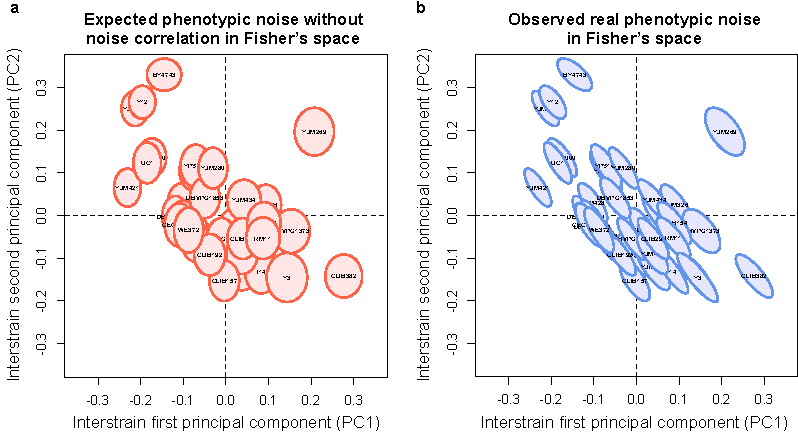
\includegraphics[scale=1]{part1_fig1.pdf}
\end{adjustwidth}
\caption[Yeast intra-strain phenotypic noise is correlated in Fisher's space.]{
\textbf{Yeast intra-strain phenotypic noise is correlated in Fisher's space.}
A singular value decomposition (SVD) is performed on the mean trait values of each of the 37 yeast strains. This space is similar to the phenotypic space used in Fisher's geometric model, where phenotypic characters mutate independently and with the same amplitude (\textit{i.e.} mean phenotype mutations are isotropic in this space). For this reason, we called this space ``Fisher's space''. We then projected single-cell data of each strain in this space. We identified the two Fisher's space axes showing most elevated noise correlation in mean, for all strains: they correspond to the first two components of Fisher's space (PC1 and PC2).
\textbf{a,} Expected phenotypic noise for each strain without noise correlation between Fisher's space axes (each axis representing a linear combination of phenotypic characters). The shape of the phenotypic noise of each strain is symbolized by an ellipse representing the standard deviation of the associated bivariate normal law. Each ellipse is tagged with the corresponding strain name. The size of the ellipses are rescaled by a factor 0.002 to better distinguish them. The coordinates of the center of each ellipse correspond to the real position of the corresponding strain in the Fisher's space (from real data).
\textbf{b,} Real observed phenotypic noise is represented, showing noise correlation between PC1 and PC2 axes, for all the strains.
}
\label{part1:fig1}
\end{figure}

For example on Figure \ref{part1:fig1}a, we show what would be an uncorrelated phenotypic noise for each strain for the two first principal components (PC1 and PC2) of the Fisher's space (the shape of the phenotypic noise of each strain is symbolized by an ellipse representing the standard deviation of the associated bivariate normal law, rescaled by a factor 0.002). On Figure \ref{part1:fig1}b, the real observed phenotypic noise is represented, showing noise correlations for all the strains. The most variable combinations of phenotypic characters (following PC1 and PC2 axes) between strains are also those exhibiting the most correlated intra-strain phenotypic noise. Thus, if one assume that phenotypic differences across strains are adaptive, our result suggests that the phenotypic characters most exposed to directional selection are also the ones with the most correlated phenotypic noise between characters.

Our analysis is described in details in Appendix \ref{part1:AppendixS1}, in Data \ref{part1:DataS1} in Data \ref{part1:DataS2}, and in Script \ref{part1:ScriptS2}.

%%%%%%%%%%%%%%%%%%%%%%%%%

\subsection{Analytical and numerical study of {\sigmaFGM}}

Our analytical and numerical approach followed three steps, as presented in Figure \ref{part1:fig2}. \textbf{(1)} We first studied {\sigmaFGM} in the case of organisms evolving a single phenotypic character, in order to evaluate previous statements \citep{zhang-et-al-2009,eldar-and-elowitz-2010,bodi-et-al-2017} (Fig. \ref{part1:fig2}a). \textbf{(2)} We then studied {\sigmaFGM} for more complex phenotypes when the phenotypic noise is isotropic, to test whether the fitness benefit of phenotypic noise for a single character is maintained for higher phenotypic complexity (Fig. \ref{part1:fig2}b). \textbf{(3)} Finally, we studied analytically and numerically the most general case in {\sigmaFGM}, where noise amplitudes on each character, as well as noise correlations between characters are evolvable, as suggested by our analysis of the phenomic data provided by \cite{yvert-et-al-2013} and by the experimental study by \cite{cressler-et-al-2017} (Fig. \ref{part1:fig2}c).

\begin{figure}[!h]
\begin{adjustwidth}{-0in}{0in}
\centering
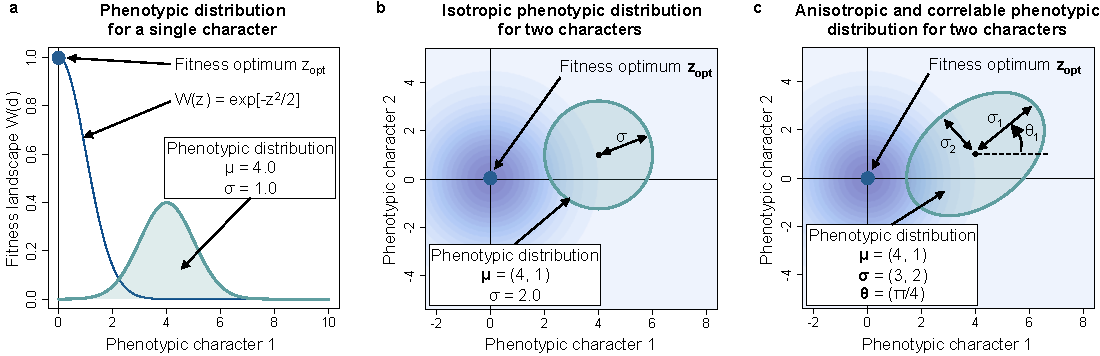
\includegraphics[width=1\linewidth]{part1_fig2.pdf}
\end{adjustwidth}
\caption[Three successive approaches to model phenotypic noise in Fisher's geometric model.]{
\textbf{Three successive approaches to model phenotypic noise in Fisher's geometric model.}
\textbf{a,} Example of an evolvable phenotypic noise on a single phenotypic character ($n=1$). $\mu=4$ and $\sigma=1$ (black box). The phenotypic distribution follows $z \sim \mathcal{N}(\mu,\sigma^2)$ (blue area). The one-dimensional fitness landscape $W(z)=\exp\left[-z^2/2\right]$ is represented in dark blue (dark blue dot: fitness optimum at $z_{opt} = 0$).
\textbf{b,} Example of an evolvable isotropic phenotypic noise on two phenotypic characters ($n=2$). $\boldsymbol{\mu} = (4,1)^T$ and $\sigma=2$ (black box). The standard deviation of the bivariate and isotropic phenotypic distribution is represented by the disc colored in blue. The fitness landscape $W(\boldsymbol{z})$ is represented by a gradient of blue (dark blue dot: fitness optimum at $\boldsymbol{z_{opt}} = (0,0)^T$).
\textbf{c,} Example of an evolvable anisotropic and correlated phenotypic noise on two phenotypic characters ($n=2$).  $\boldsymbol{\mu} = (4,1)^T$, $\boldsymbol{\sigma} = (3,2)^T$ and $\boldsymbol{\theta} = (\pi/4)$ (black box). The standard deviation of the bivariate phenotypic distribution is represented by the blue ellipse colored in blue. The fitness landscape $W(\boldsymbol{z})$ is represented by a gradient of blue (dark blue dot: fitness optimum $\boldsymbol{z_{opt}} = (0,0)^T$).
}
\label{part1:fig2}
\end{figure}

%%%%%%%%%%%%%%%%%%%%%%%%%

\subsubsection{Elevated phenotypic noise is beneficial in directional selection for a single phenotypic character.}

We first studied {\sigmaFGM} in the simple case of the evolution of a single phenotypic character. The phenotypic noise is then reduced to an univariate normal law $\mathcal{N}(\mu,\sigma^2)$, with $\mu$ the single mean trait value and $\sigma$ the standard deviation of the phenotypic noise on this character (Fig. \ref{part1:fig2}a). To understand what would be the selective pressures on $\mu$ and $\sigma$ in the phenotypic space, we analytically studied the sub-population fitness $\overline{W}(\mu,\sigma)$, under the hypothesis of an infinite population (Eq. \ref{eq:integrative_fitness}). The mathematical details of our analytical and numerical approaches are presented in Appendix \ref{part1:AppendixS2} and Appendix \ref{part1:AppendixS3}. Figure \ref{part1:fig3} shows that, if evolvable, phenotypic noise should increase during directional selection, and then decrease when selection becomes stabilizing, as predicted in \cite{eldar-and-elowitz-2010}.
When the population is far from the fitness optimum $z_{opt}$, it is beneficial to increase the phenotypic noise (Fig. \ref{part1:fig3} green area). On the contrary, when the population is near the fitness optimum, or when noise amplitude is too high, it is better to decrease phenotypic noise, as shown in previous studies \citep{mineta-et-al-2015,keren-et-al-2016} (Fig. \ref{part1:fig3} red area).

\begin{figure}[!ht]
\centering
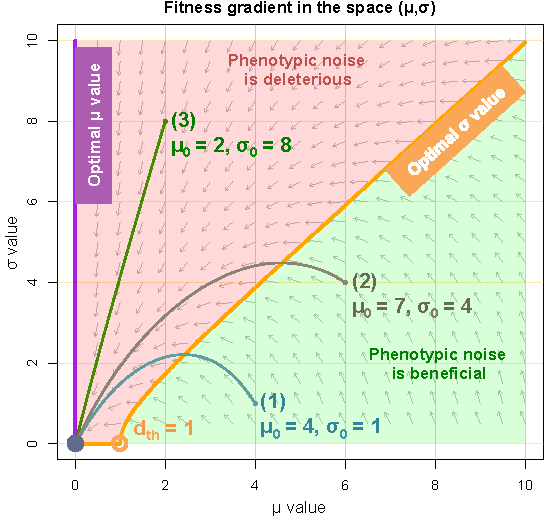
\includegraphics[scale=1]{part1_fig3.pdf}
\caption[Variations of the sub-population fitness $\overline{W}(\mu,\sigma)$ depending on $\mu$ and $\sigma$ values.]{\textbf{Variations of the sub-population fitness $\overline{W}(\mu,\sigma)$ depending on $\mu$ and $\sigma$ values.}
Following the purple curve, the optimal $\mu$ value given a $\sigma$ value. Following the orange curve, the optimal $\sigma$ value given a $\mu$ value. Green area: it is beneficial to increase the phenotypic noise. Red area: it is beneficial to reduce the phenotypic noise. Three trajectories following the fitness gradient are represented \textbf{(1)} in blue (initial values: $\mu_0=4, \sigma_0=1$), \textbf{(2)} in brown (initial values: $\mu_0=6, \sigma_0=4$) and \textbf{(3)} in green (initial values: $\mu_0=2, \sigma_0=8$). Black dot: fitness optimum $z_{opt}$. Orange circle: inflection point $d_{th}=1$ of the fitness landscape $W(z)$. Grey arrows indicate the direction of the fitness gradient, but not its amplitude.
}
\label{part1:fig3}
\end{figure}

Thus, depending on the euclidean distance from the fitness optimum, there exists an optimal value of $\sigma$ giving the highest fitness value, as shown by the orange curve on Figure \ref{part1:fig3}. At the critical distance $d_{th} = 1$ (Fig. \ref{part1:fig3} orange circle, Appendix \ref{part1:AppendixS3}), which corresponds to the inflection point of the fitness function $W(z)$ \citep{zhang-et-al-2009}, phenotypic noise is always deleterious and must be minimized by organisms. However, reducing the euclidean distance from the fitness optimum is always beneficial, whatever the value of $\sigma$, as shown by the purple curve on Figure \ref{part1:fig3}. As exemplified by trajectories \textbf{(1)}, \textbf{(2)} and \textbf{(3)} on Figure \ref{part1:fig3}, a population adapting to the new fitness optimum (Fig. \ref{part1:fig3} dark blue dot) will increase or decrease its phenotypic noise depending on initial conditions. The prediction of \cite{eldar-and-elowitz-2010} corresponds to trajectory \textbf{(1)}, \textit{e.g.}, when a population anciently in stabilizing selection (with reduced phenotypic noise) must adapt to a new environment. Trajectories \textbf{(2)} and \textbf{(3)} could correspond \textit{ e.g.}, to a single stress-related gene, with elevated phenotypic noise at the moment of the environmental shift.

Then, in the case of a population evolving a single phenotypic character, our results confirm the claim that phenotypic noise is beneficial in directional selection, when the population is far from the fitness optimum, and that phenotypic noise is deleterious in stabilizing selection, when the population reaches the fitness optimum \citep{eldar-and-elowitz-2010}. As previously demonstrated by \cite{zhang-et-al-2009}, a condition to the positive selection of phenotypic noise is the existence of a convex fitness landscape. In a recent experimental study on \textit{Saccharomyces cerevisiae}, \cite{keren-et-al-2016} suggest that it could be the case for many traits.

%%%%%%%%%%%%%%%%%%%%%%%%%

\subsubsection{There is a cost of complexity on isotropic phenotypic noise in directional selection}

When organisms evolve a single phenotypic character, {\sigmaFGM} is in accordance with previous results \citep{zhang-et-al-2009,eldar-and-elowitz-2010,bodi-et-al-2017}. However, the fitness effect of phenotypic noise is unclear when the phenotypic complexity increases, since the evolution of phenotypic noise can potentially be impeded by a cost of complexity, as defined by \cite{fisher-1930}. To address this question, we first generalized the one-dimensional case by increasing the number of phenotypic characters, but keeping an isotropic phenotypic noise (similar to a ``global'' phenotypic noise affecting the whole phenotype, \citealt{yvert-et-al-2013}). An isotropic noise is applied to the mean phenotype $\boldsymbol{\mu}$ of an organism, by independently varying each trait value $\mu_i$ with the same amplitude $\sigma$ (Fig. \ref{part1:fig2}b).
In {\sigmaFGM}, this scenario corresponds to constrain the evolution of the covariance matrix $\boldsymbol{\Sigma}$ such that $\boldsymbol{\Sigma} = \sigma^2 \boldsymbol{I_n}$, and to remove noise correlations ($\boldsymbol{\theta} = \boldsymbol{0}$).
We repeated the analysis made for a single phenotypic character, but ranging from a single to 50 characters. The details of our analytical and numerical approaches are presented in Appendix \ref{part1:AppendixS2} and Appendix \ref{part1:AppendixS3}.

The results, presented in Figure \ref{part1:fig4}, show that the advantage of an isotropic phenotypic noise is quickly impeded when the phenotypic complexity increases. First, the euclidean distance $d_{th}$ below which phenotypic noise is deleterious increases with the phenotypic complexity. An analytical resolution shows that $d_{th}$ increases as the square root of the number of phenotypic characters ($d_{th} = \sqrt{n}$, Fig. \ref{part1:fig4}a, and Appendix \ref{part1:AppendixS3}).
Second, the fitness gain brought by an optimal phenotypic noise (Fig. \ref{part1:fig4}a orange and grey curves) quickly vanishes with phenotypic complexity. Indeed, when organisms have more than one phenotypic characters ($n>1$), the beneficial value of phenotypic noise becomes rapidly negligible (Fig. \ref{part1:fig4}b). The maximal fitness gain when phenotypic noise is optimal also rapidly falls down, with \textit{e.g.}, a maximal fitness gain for two characters ($n=2$) representing only $\sim36\%$ of the maximal gain for a single character (Fig. \ref{part1:fig4}b black dots).

These results show that predictions based on the evolution of a single character cannot be generalized as is at the level of the phenotype, when the phenotypic noise is isotropic, as it undergoes a cost of complexity.

\begin{figure}
\centering
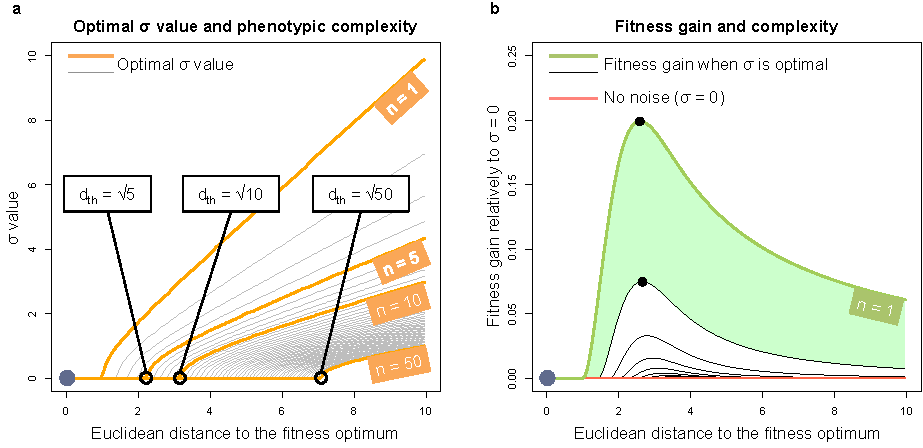
\includegraphics[scale=1]{part1_fig4.pdf}
\caption[Effects of phenotypic complexity on isotropic phenotypic noise fitness gain.]{\textbf{Effects of phenotypic complexity on isotropic phenotypic noise fitness gain.}
\textbf{a,} Variation of the optimal $\sigma$ value, depending on the euclidean distance. $x$ axis: the euclidean distance from the fitness optimum is varied from 0 to 10, for all phenotypic complexities ($d=\lVert \boldsymbol{\mu} \rVert$). $y$ axis: the amplitude $\sigma$ of the phenotypic noise is varied from 0 to 10. Grey curves: optimal $\sigma$ value for each phenotypic complexity. Phenotype complexities $n=1$, $n=5$, $n=10$ and $n=50$ are highlighted in orange. Black circle: the critical euclidean distance $d_{th}$ below which phenotypic noise is always deleterious is equal to $\sqrt{n}$ (exemplified here for $n=5$, $n=10$ and $n=50$).
\textbf{b,} Fitness gain when $\sigma$ is optimal, compared to canonical FGM scenario with no phenotypic noise ($\sigma = 0$). Dark blue dot: fitness optimum. Black curves: fitness gain when isotropic noise is optimal. Phenotypic complexity $n=1$ is highlighted in green. The green area indicates the difference of fitness gain between $n=1$ and $n=2$. Red line: no fitness gain (no phenotypic noise scenario). Black dots: maximal fitness gains when $n=1$ and $n=2$. The maximal fitness gain of isotropic noise when $n=2$ represents $\sim36\%$ of the maximal gain for a single character.
}
\label{part1:fig4}
\end{figure}

%%%%%%%%%%%%%%%%%%%%%%%%%

\subsubsection{Anisotropic and correlated phenotypic noise is beneficial when aligned with the fitness optimum}

Finally, we studied the most general case in {\sigmaFGM}, as described in Methods. Noise amplitude on each character, as well as noise correlations between characters are evolvable (Fig. \ref{part1:fig2}c). As a first step, we analyzed the model in a static situation, with no mutational process (as for previous results), in order to guess what would be the selective pressures on the phenotypic noise.

We show mathematically (Appendix \ref{part1:AppendixS3}) that when the population is far from the fitness optimum, the best configuration (\textit{i.e.}, the one that gives the best fitness advantage) is a flattened, one-dimensional phenotypic noise, with elevated noise in the direction of the fitness optimum and no noise in all other directions. Any other form of phenotypic noise (isotropic or not perfectly aligned with the fitness optimum) gives a lower sub-population fitness $\overline{W}(\boldsymbol{\mu},\boldsymbol{\Sigma})$. This does not mean that a badly aligned phenotypic noise is deleterious for organismal fitness, compared to an organism with no phenotypic noise for example. As shown in Figure \ref{part1:fig4}, even an isotropic noise slightly increases the fitness when the population is far from the fitness optimum. However, as also shown in Figure \ref{part1:fig4}, the best fitness gain is obtained when the phenotypic noise is one-dimensional. Similarly, the best phenotypic noise configuration in $n$ dimensions consists in a dimensionality reduction to fight the cost of complexity on phenotypic noise. A population evolving such a phenotypic noise will recover the benefit of a single character scenario, phenotypic noise conferring a strong fitness advantage to organisms in directional selection (Figs. \ref{part1:fig3} and \ref{part1:fig4}).
The mathematical demonstration of this result is provided in Appendix \ref{part1:AppendixS3}.

%%%%%%%%%%%%%%%%%%%%%%%%%

\subsubsection{Evolvable anisotropic and correlated phenotypic noise compensates for the cost of complexity in directional selection}

To test our mathematical prediction on the evolution of an anisotropic and correlated phenotypic noise (see above), we used a numerical scheme to compute the evolutionary trajectory of an initially maladapted population towards the fitness optimum. To do so, we estimated the evolution of the population distribution $n(\boldsymbol{\mu},\boldsymbol{\sigma},\boldsymbol{\theta})$ through time by simulating the stochastic branching process in finite population associated to the model, as described in Methods.

In directional selection and with a complex phenotype, if organisms are allowed to evolve a correlated phenotypic noise, will they do so? And if yes, what will be the consequence on the evolution speed depending on phenotypic complexity? To address these questions, we measured the convergence time to the fitness optimum of an evolving population in four different scenarios:
\begin{enumerate}
\item[\textbf{(1)}] The mutation sizes $s_\sigma$ and $s_\theta$ of the phenotypic noise parameters $\boldsymbol{\sigma}$ and $\boldsymbol{\theta}$ are lower than for $s_\mu$ ($s_\mu = 0.01, s_\sigma = s_\theta = 0.001$);
\item[\textbf{(2)}] The mutation sizes $s_\sigma$ and $s_\theta$ are equal to the mutation size $s_\mu$ ($s_\mu = s_\sigma = s_\theta = 0.01$);
\item[\textbf{(3)}] The mutation sizes $s_\sigma$ and $s_\theta$ are higher than $s_\mu$ ($s_\mu = 0.01, s_\sigma = s_\theta = 0.1$).
\item[\textbf{(4)}] Organisms have no phenotypic noise, as in canonical FGM ($s_\mu = 0.01, s_\sigma = s_\theta = 0.0$, and $\boldsymbol{\sigma}=\boldsymbol{0}, \boldsymbol{\theta}=\boldsymbol{0}$)
\end{enumerate}

The simulations were computed for a phenotypic complexity ranging from $n=1$ to $n=10$. 100 repetitions have been computed per parameter set. The population was considered to have converged towards the optimum when the mean fitness of the population was higher than 0.9.
All populations were initialized with a very low level of phenotypic noise ($\boldsymbol{\sigma} \sim \boldsymbol{0}$), and no rotation of the covariance matrix $\boldsymbol{\Sigma}$ ($\boldsymbol{\theta} = \boldsymbol{0}$). The initial euclidean distance was $d_{init} = 4.0$ for all the simulations (beyond the critical distance $d_{th} = \sqrt{n}$, see above). To do so, the $\mu_i$ values of the initial mean phenotype $\boldsymbol{\mu}$ were set to $\mu_i = d_{init}/\sqrt{n}$.
To keep the mutation sizes constant whatever the phenotypic complexity, $s_\mu$, $s_\sigma$ and $s_\theta$ were also normalized by $\sqrt{n}$.

To facilitate the analysis of numerical outputs, we used three different measures:
\begin{enumerate}
\item[\textbf{(1)}] The \textit{maximal eigenvalue} indicates the amount of phenotypic noise on the distribution $\mathcal{N}_n(\boldsymbol{\mu},\boldsymbol{\Sigma})$ (Eq. \ref{eq:phenotypic_noise}), and is equal to $\max(\boldsymbol{\sigma}^2)$;
\item[\textbf{(2)}] The \textit{maximal eigenvalue contribution} indicates the contribution of the maximum eigenvalue to the total amount of noise. It is obtained by computing:
\begin{equation}
\dfrac{\max(\boldsymbol{\sigma}^2)}{\sum\limits_{i \in n} \sigma_i^2};
\label{eq:maximum_eigenvalue_contribution}
\end{equation}
\item[\textbf{(3)}] The \textit{maximal eigenvector correlation} is the correlation (dot product) between the eigenvector associated to the maximal eigenvalue, and the direction of the optimum. If the correlation $\approx 1$, the principal axis of the phenotypic distribution is aligned towards the optimum. If the correlation $\approx 0$, the principal axis is orthogonal to the direction of the optimum (by symmetry, we take the absolute value of the dot product).
\end{enumerate}

\begin{figure}[!h]
\begin{adjustwidth}{-0in}{0in}
\centering
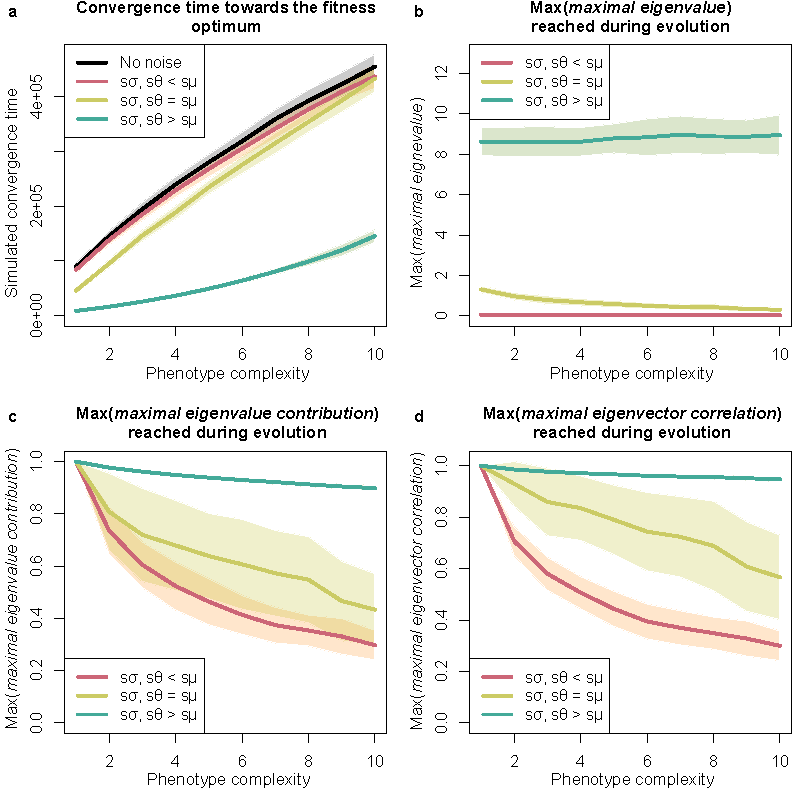
\includegraphics[scale=1]{part1_fig5.pdf}
\end{adjustwidth}
\caption[An evolvable anisotropic and correlated phenotypic noise speeds up evolution.]{\textbf{An evolvable anisotropic and correlated phenotypic noise speeds up evolution.}
\textbf{a,} Convergence time towards the fitness optimum. Four scenarios are evaluated. Black curve: canonical FGM scenario, with no phenotypic noise. Colored curves: evolvable phenotypic noise scenarios. $x$-axis: phenotypic complexity, from $n=1$ to $n=10$. $y$-axis: Convergence time.
\textbf{b, c, d,} Maximum values of \textbf{b,} the \textit{maximum eigenvalue} ($max(\boldsymbol{\sigma})$), \textbf{c,} the \textit{maximum eigenvalue contribution} (Eq. \ref{eq:maximum_eigenvalue_contribution}), and \textbf{d,} the \textit{maximum eigenvalue dot product} (with the direction of the fitness optimum) reached by the population during its evolution towards the fitness optimum, respectively. Four scenarios are evaluated (legends): three with evolvable phenotypic noise, one with no phenotypic noise (canonical FGM scenario). For each scenario, the mean (colored lines) and the standard deviation along the 100 repetitions (shaded areas) are represented. In all cases, the scenario where $s_\sigma, s_\theta >  s_\mu$ is characterized by the evolution of a near perfectly flattened and one-dimensional phenotypic noise, fully aligned with the fitness optimum, as predicted mathematically.
}
\label{part1:fig5}
\end{figure}

For each numerical simulation, both the mean and the variance of these measures have been computed along the 100 repetitions, at each time-step. As shown in Figure \ref{part1:fig5}, an evolvable phenotypic noise speeds up evolution, whatever the phenotypic complexity (Fig. \ref{part1:fig5}a). However, this gain depends on the mutation size of phenotypic noise parameters ($s_\sigma$ and $s_\theta$) relative to the mutation size of the mean trait values ($s_\mu$). If $s_\sigma$ and $s_\theta$ are lower or equal to $s_\mu$, the fitness gain is low (Fig. \ref{part1:fig5}a). If $s_\sigma$ and $s_\theta$ are higher than $s_\mu$, the evolution speed gain is significant, with a convergence time much lower than for canonical FGM scenario (with no phenotypic noise), whatever the phenotypic complexity.
The analysis of the three measures indicates that a cost of complexity exists on the evolution of the phenotypic noise, such that if $s_\sigma, s_\theta \leq s_\mu$, the phenotypic noise does not have the time to evolve towards a one-dimensional shape (with elevated noise in the direction of the fitness optimum, and no noise in all other directions). For each measure (the maximum eigenvalue, its contribution and its dot product), the maximum value reached during a simulation is plotted against the phenotypic complexity, for each of the four scenarios (Figs. \ref{part1:fig5}b,c,d). This maximum value represents the efficacy of evolution in shaping the phenotypic noise in directional selection, knowing that noise increases when the population is far from the fitness optimum, and then decreases when the population reaches the fitness optimum.
A trade-off seems to exist between the convergence time of the mean phenotype $\boldsymbol{\mu}$ and the time needed for evolution to shape the phenotypic noise. On Figure \ref{part1:fig5}b, we see that the maximum eigenvalue does not reach the optimal value $\approx 9.0$ when $s_\sigma, s_\theta \leq s_\mu$. However, when $s_\sigma, s_\theta > s_\mu$, the maximum eigenvalue reaches the optimal value whatever the phenotypic complexity. Indeed, in this situation organisms have time to evolve the most beneficial, flattened form of phenotypic noise.
On Figures \ref{part1:fig5}c and \ref{part1:fig5}d, the maximum eigenvalue contribution and the maximum eigenvalue dot product are strongly lessened with phenotypic complexity when $s_\sigma, s_\theta \leq s_\mu$, while they are almost equal to 1 whatever the phenotypic complexity when $s_\sigma, s_\theta > s_\mu$. In the latter case, the phenotypic noise evolves towards a near perfect flattened form, as predicted previously, hence strongly speeding up adaptation.

%%%%%%%%%%%%%%%%%%%%%%%%% SECTION : DISCUSSION %

\section{Discussion}

The fitness benefit of elevated phenotypic noise in directional selection was foreseen by \cite{eldar-and-elowitz-2010}, who stated that ``\textit{one might expect increased phenotypic noise during periods of adaptation to new environments, followed by reduction in noise when selection becomes stabilizing}''. Based on a mathematical model, \cite{zhang-et-al-2009} also stated that elevated noise would increase the probability to fix beneficial mutations in directional selection, provided that the local fitness landscape is convex. This prediction has been corroborated in a recent experimental study on the evolution of a single gene in \textit{Saccharomyces cerevisiae} \citep{bodi-et-al-2017}. However, these results are based on the evolution of a single phenotypic character, while real phenotypes are much more complex, with multiple characters under selection. We extended Fisher's geometric model \citep{fisher-1930} to account for evolvable phenotypic noise, in order to address the question of how phenotypic noise would evolve in directional selection, when organisms own complex phenotypes. This model, named {\sigmaFGM}, allows for evolvable phenotypic noise amplitudes on each character, but also for evolvable noise correlations between characters, as justified by our analysis of the phenomic data of \cite{yvert-et-al-2013}, and an experimental study by \cite{cressler-et-al-2017}.

First, we studied analytically the case where organisms own a single phenotypic character, and must evolve towards a novel environment. Doing so, we confirmed previous results \citep{zhang-et-al-2009,eldar-and-elowitz-2010,bodi-et-al-2017}: elevated phenotypic noise is beneficial under directional selection, when the population is far from the fitness optimum and experiences a convex fitness landscape. When the population is near the fitness optimum, the phenotypic noise is deleterious and must be minimized, confirming previous statements that phenotypic noise is deleterious under stabilizing selection \citep{mineta-et-al-2015,keren-et-al-2016}.

In 1930, \cite{fisher-1930} hypothesized that organisms evolving towards a fitness optimum experience a cost of complexity, beneficial mutations becoming increasingly harder to fix when the number of phenotypic characters under selection increases. Here, we demonstrated that this cost of complexity also hinders the benefit of an elevated phenotypic noise in directional selection, when noise is isotropic. In this case, when the number of phenotypic characters is higher than one, the beneficial fitness effect of phenotypic noise quickly vanishes. Moreover, the critical distance from the fitness optimum below which the phenotypic noise must be minimized increases as the square root of the number of characters, suggesting that for a constant distance from the fitness optimum, more complex organisms are expected to be less noisy.

Recent studies suggested that phenotypic noise could be considered as a complex phenotypic character, possibly tuned by the genotype-to-phenotype map \citep{yvert-et-al-2013,boukhibar-and-barkoulas-2016}, and correlated \citep{cressler-et-al-2017}. Here, we demonstrated that under directional selection on a convex fitness landscape, the best possible configuration for the phenotypic noise is to evolve towards a flattened, one-dimensional configuration, with elevated noise in the direction of the fitness optimum, and no noise in all other directions. In this case, the evolving population recovers the beneficial value of an elevated phenotypic noise, as for the single phenotypic character scenario. We also demonstrated that in this specific configuration, phenotypic noise increases the probability to fix beneficial mutations and accelerates evolution, whatever the phenotypic complexity, thereby partly compensating for the cost of complexity. To be fully exploitable by evolution, the properties of the phenotypic noise must evolve at a higher speed than the mean phenotype. However, it is not required for the noisy phenotype to be inherited in our model, suggesting that when it is the case \citep{charlebois-et-al-2011}, this constraint could be relaxed.

Our findings are in accordance with recent experimental results. First, \cite{cressler-et-al-2017} demonstrated the existence of correlated phenotypic noise on \textit{Daphnia pulicaria} (a freshwater zooplankton). By measuring three integrated phenotypic characters at the individual level (body growth, number of eggs and longevity) on different populations of genetic variants, they showed that there are no significant genetic correlations between characters, while there is strong evidence for positive non-genetic correlations between characters. Moreover, they showed that increasing phenotypic noise enhances growth rate when non-genetic correlations between characters are positive, in agreement with our prediction on the evolution of phenotypic noise. Second, our analysis of single-cell yeast data provided by \cite{yvert-et-al-2013} revealed that the phenotypic characters showing the strongest noise correlations are also the most variables between strains, suggesting that a correlated phenotypic noise evolved on the phenotypic characters most exposed to directional selection (Appendix \ref{part1:AppendixS1}). Finally, an experimental study by \cite{metzger-et-al-2015} suggested that the expression noise of TDH3 gene may evolve faster than its mean expression, suggesting that it could be the case for phenotypic noise in general, in agreement with our findings.

As a whole, our results show that such non-isotropic phenotypic noise could be exploited by evolution, and suggest further experiments to assess the functional nature of phenotypic noise. In particular, phenotypic noise has been demonstrated to have a role in drug resistance \citep{singh-et-al-2010,charlebois-et-al-2014,charlebois-2015}, cancer cells proliferation \citep{gascoigne-taylor-2008,cohen-et-al-2008,huang-2012,pisco-et-al-2013} as well as in the process of decision-making, seen as an adaptation to a environmental change \citep{richard-et-al-2016}. It could be interesting to initiate new experiments letting biological populations adapt to a novel environment, and acquire phenotypic noise data at the individual level \citep{ohya-et-al-2015}. The long-term evolution experiment (LTEE, \citealt{elena-and-lenski-2003}), where populations of \textit{Escherichia coli} are evolved in a minimum glucose medium since more than 66,000 generations, and regularly frozen to keep track of evolution, would be a good candidate to initiate such an experiment. Moreover, our predictions on the evolution of phenotypic noise in directional selection could be used to predict the future direction of evolution, and to localize the fitness optimum in the phenotypic space. Indeed, tracking the evolution of phenotypic noise experimentally could help biologists understand what are the selective pressures at work on organisms, and to anticipate the next evolution steps.

By extending Fisher's geometric model with evolvable phenotypic noise, we offered general predictions on what would be the evolution of phenotypic noise in directional selection, and its consequences on the fate of asexual populations experiencing directional selection.
Our demonstrations rely on the assumption that the phenotypic noise and the fitness landscape are Gaussian-shaped, as it is historically the case in Fisher's geometric model. If the phenotypic noise is not Gaussian, other particular cases could appear, even if locally there is always a benefit to be noisy in directions where the fitness is convex. By relaxing our hypotheses, other interesting questions could be tackled, for example the case where the fitness landscape is multimodal or not static, the case of a degenerated noise (\textit{e.g.}, where some directions in the phenotypic space are forbidden), or whether the case of a multiplicative noise. By deciphering the conditions in which phenotypic noise evolves towards specific patterns, our results may contribute to the growing field of predictive biology.

\newpage

%%%%%%%%%%%%%%%%%%%%%%%%% SECTION : SUPPORTING INFORMATION %

\section{Supporting Information}

%%%%%%%%%%%%%%%%%%%%%%%%%%%

\subsection{Figure S1. An example of the temporal dynamics in {\sigmaFGM}.}
\label{part1:FigureS1}

\begin{figurehere}
\begin{adjustwidth}{-0in}{0in}
\centering
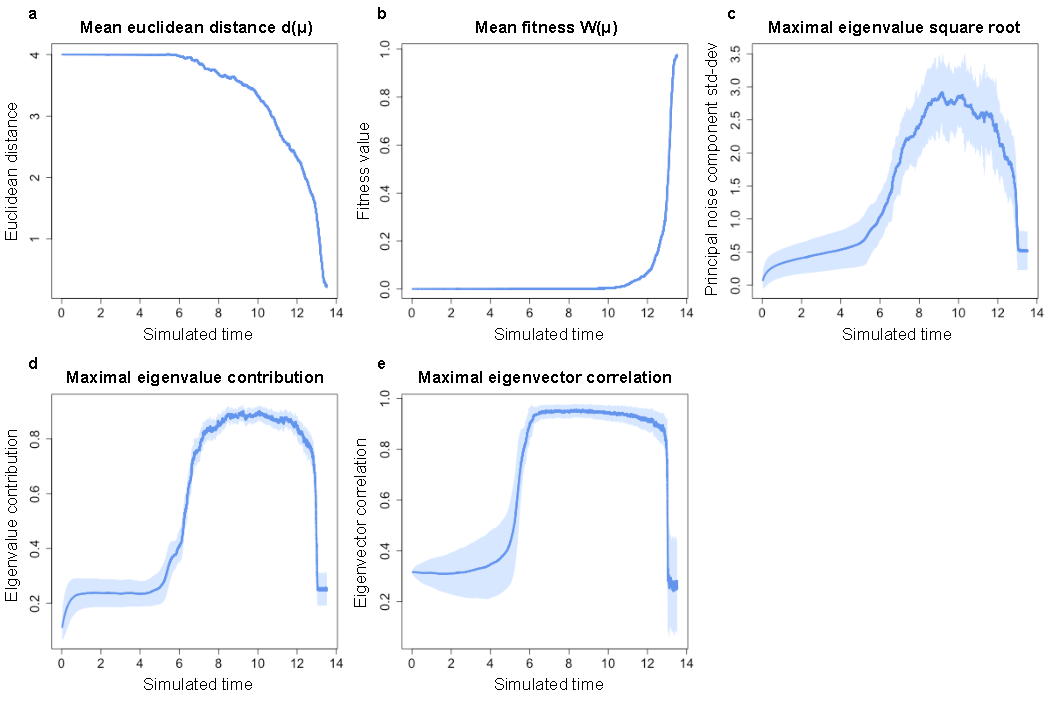
\includegraphics[width=1\linewidth]{part1_figS1.pdf}
\end{adjustwidth}
\caption[An example of the temporal dynamics in {\sigmaFGM}.]{
\textbf{An example of the temporal dynamics in {\sigmaFGM}.}
A simulation in $n=10$ dimensions is initialized with 10,000 organisms having the same triplet $(\boldsymbol{\mu}_0, \boldsymbol{\sigma}_0, \boldsymbol{\theta}_0)$, with $\boldsymbol{\mu}_0 = \{4.0/\sqrt{n}\}^T$, $\boldsymbol{\sigma}_0=\boldsymbol{0}$, and $\boldsymbol{\theta}_0=\boldsymbol{0}$. The initial population is then localized on the hyper-sphere of radius 4.0, none of the phenotypic characters being aligned with the fitness optimum $z_{opt}$, and thus requiring to be adapted. $s_\mu=0.01$, and $s_\sigma=s_\theta=0.1$. The simulation stopped when the population mean of the mean fitness $\langle W(\boldsymbol{\mu}) \rangle$ reached 0.9.
\textbf{a,} The population mean of the mean euclidean distance $\langle d(\boldsymbol{\mu}) \rangle$.
\textbf{b,} The population mean of the mean fitness $\langle W(\boldsymbol{\mu}) \rangle$.
\textbf{c,} The population mean of the maximal eigenvalue.
\textbf{d,} The population mean of the maximal eigenvalue contribution.
\textbf{e,} The population mean of the maximal eigenvector correlation with the direction of the fitness optimum.
The standard deviation of each variable is represented by a shaded blue area.
}
\label{figS1}
\end{figurehere}

\newpage

%%%%%%%%%%%%%%%%%%%%%%%%%%%

\subsection{Appendix S1. Various wild-types of yeast exhibit correlated phenotypic noise.}
\label{part1:AppendixS1}


In this appendix, we present the results of our analysis on the experimental single-cell data provided by \cite{yvert-et-al-2013}. We assume that the reader is aware of the basic definitions and equations provided in the main manuscript.

\cite{yvert-et-al-2013} used automated image analysis to describe yeast phenotypic diversity at a single-cell resolution (known as phenomics, \citealt{ohya-et-al-2015}). They monitored $n=125$ phenotypic characters on isogenic populations of $m=37$ different strains of yeast, living in natural or laboratory conditions. For each strain, they measured 5 replicates of approximately 200 cells each ($\sim$1000 cells per strain). They demonstrated that phenotypic noise significantly differs between strains, supporting ``\textit{the possibility that, if noise is adaptive, microevolution may tune it in the wild}'' \citep{yvert-et-al-2013}.

We used the raw datasets published by the authors to measure intra-strain (\textit{i.e.} isogenic) noise correlations between characters. The goal of our study is to test the existence of correlated phenotypic noise in natural strains of yeast. The datasets provided by \cite{yvert-et-al-2013} are structured as following: for each strain of yeast, a set of files is provided in a dedicated folder (a dataset per replicate). For each replicate, the list of single-cell measures is dispatched in three different files in \texttt{xls} format. Each cell is identified by a unique tag per image and the tag of the captured image. Each time a measure failed (on one character, or on the entire cell), the corresponding element (or line) in the table was filled with value $-1$.
Several characters are redundant (for example the volume and the size of the nucleus), and strongly correlated. Moreover, each trait value is provided with specific units (\textit{e.g.}, number of pixels, volume or angle units), such that some normalization is necessary.
The code associated to this analysis is freely available in Script \ref{part1:ScriptS2}. One can run again the whole analysis by following instructions provided in the README file. The raw dataset is freely provided by \cite{yvert-et-al-2013}.

The purpose of the analysis is to determine whether intra-strain variability presents correlations between characters \textit{once inter-strain correlations  between characters have been removed}. 

Let us first process inter-strain variability. The idea is to find a phenotypic space in which there is as little character-specific variability and correlation as possible. Here we have 37 isogenic strains, hence 37 genotypes. We define the ``phenotype'' of a strain/genotype as the vector of mean trait values, computed over all cells from this strain/genotype. We then define the ``centered phenotype" of a strain/genotype by removing the grand mean of each character. The singular value decomposition of the 37x125 matrix of centered strain phenotypes will give us a set of orthonormal linear combinations of characters. By construction, when the centered strain phenotypes are expressed according to these new characters, they lose all their pairwise correlations, implying that the variance-covariance matrix is diagonal for those new characters. Moreover, we normalize the variance of each new strain phenotype to one\footnote{Which is why our analysis is not exactly a PCA: We drop the singular values that are usually left in the PCA.}, such that the 37 new strain phenotypes are isotropically distributed.

This new base is the closest analogy we could think of to the phenotypic space in the classical version of Fisher's geometric model. Fisher's phenotypic space is orthogonal and normalized, and mutations on the genotype cause phenotypic traits to vary independently and with the same amplitude, according to an isotropic mutational distribution.

The second step is to project intra-strain single-cell data in Fisher's space, and to analyze the possible remaining correlations of intra-strain phenotypic variability in this space.

Figure \ref{part1:appendixS1:fig1} shows the detailed steps of our analysis, as described  below. First, we converted each \texttt{xls} file into \texttt{csv} format, and we merged the three files of each replicate to obtain a single dataset $\boldsymbol{M_{0,s,r}}$ ($s \in \{1,...,37\}$, $r \in \{1,...,5\}$) per replicate, and we removed useless information (such as cell identifiers, coordinates on the image, and so on) (Fig. \ref{part1:appendixS1:fig1}.1).
Then we merged the 5 replicates of each strain (Fig. \ref{part1:appendixS1:fig1}.2) to compute the matrix $\boldsymbol{M_0}$ of the mean phenotypic characters per strain (Fig. \ref{part1:appendixS1:fig1}.3).
Each column ${\boldsymbol{M_0}}_j$ of $\boldsymbol{M_0}$ was centered and normalized to obtain the matrix $\boldsymbol{M}$ (Fig. \ref{part1:appendixS1:fig1}.4):
\begin{equation}
{\boldsymbol{M}}_j = \dfrac{{\boldsymbol{M_0}}_j-\mathrm{mean}({\boldsymbol{M_0}}_j)}{\mathrm{stdev}({\boldsymbol{M_0}}_j)}.
\end{equation}
We also standardized each replicate to obtain $37\times5$ matrices $M_{s,r}, s \in \{1,...,37\}, r \in \{1,...,5\}$ (Fig. \ref{part1:appendixS1:fig1}.6). For each column ${\boldsymbol{M_{0,s,r}}}_j$ of $\boldsymbol{M_{0,s,r}}$:
\begin{equation}
{\boldsymbol{M_{s,r}}}_j = \dfrac{{\boldsymbol{M_{0,s,r}}}_j-\mathrm{mean}({\boldsymbol{M_{0,s,r}}}_j)}{\mathrm{stdev}({\boldsymbol{M_{0,s,r}}}_j)}.
\end{equation}
To find Fisher's space, we computed a SVD from $\boldsymbol{M}$ (see details below, and Fig. \ref{part1:appendixS1:fig1}.5).
For each standardized replicate dataset $\boldsymbol{M_{s,r}}$, many trait values are missing, and are replaced by $-1$ values, making impossible some mathematical operations. For this reason, a next step was to estimate the missing values: we used a simple conservative method, as described below (Fig. \ref{part1:appendixS1:fig1}.7). Finally, each replicate dataset was projected in Fisher's space (Fig. \ref{part1:appendixS1:fig1}.8). The inter-replicate variability was evaluated to ensure that experimental variability is low enough (Fig. \ref{part1:appendixS1:fig1}.9), and intra-strain phenotypic noise correlations were analyzed (Fig. \ref{part1:appendixS1:fig1}.10).

We describe below the steps requiring details.

%%%%%%%%%%%%%%%%%
%%%%%%%%%%%%%%%%%

\section*{Estimation of missing values}
To estimate missing values, we first computed the cell-to-cell Pearson correlation matrix $\boldsymbol{C}$ associated to each replicate, based on available data.
Knowing there are $m' \sim 200$ cells and $n=125$ phenotypic characters in each replicate, we defined a cell by a vector $\boldsymbol{X_i} \in \mathbb{R}^{125}$, with $i \in \{1,...,m'\}$.

Each missing value $x_{i,j}$ of $\boldsymbol{X_i}$ (with $j \in \{1,...,n\}$) was recovered by computing:
\begin{equation}
x_{i,j} = \bar{\boldsymbol{X_i}}+ \dfrac{\sum\limits_{k=1}^{m'} (x_{k,j}-\bar{\boldsymbol{X_k}})c_{i,k}}{\sum\limits_{k=1}^{m'} |c_{i,k}|}
\end{equation}
with $c_{i,k}$ element of $\boldsymbol{C}$. This simple method is conservative, meaning that noise amplitudes tend to be reduced through this estimation method.
Moreover, we removed all cells $X_i$ that contained only $-1$ values.

%%%%%%%%%%%%%%%%%
%%%%%%%%%%%%%%%%%

\section*{Singular value decomposition}
Let us consider the matrix $\boldsymbol{M}$ of dimension $m \times n$ that contains the standardized mean phenotypic trait values of each strain, where $m$ is the number of strains ($m=37$), and $n$ is the number of characters ($n=125$).
$\boldsymbol{M}$ can be decomposed into a $m \times m$ unitary matrix $\boldsymbol{U}$, a $m \times n$ positive and diagonal matrix $\boldsymbol{\Sigma}$, and a $n \times n$ unitary matrix $\boldsymbol{V}$ such that:
\begin{equation}
\boldsymbol{M} = \boldsymbol{U} \boldsymbol{\Sigma} \boldsymbol{V}^*
\label{eq:part1:sigmaFGM:SVD}
\end{equation}
with $\boldsymbol{V}^*$ being the conjugate transpose of $\boldsymbol{V}$.

The diagonal entries of $\boldsymbol{\Sigma}$ are the singular values $\boldsymbol{\sigma} \in \mathbb{R}^m$ of $\boldsymbol{M}$. $\boldsymbol{V}$ contains the right-singular vectors of $\boldsymbol{M}$, defining the base where $m$ linear combinations of phenotypic characters are separated and orthonormal. These linear combinations give 37 new phenotypic characters, whose means vary independently and have been normalized to the same amplitude. In the following, we will call the space generated by the base $\boldsymbol{V}$ the ``Fisher's space''.

As shown on Figure \ref{part1:appendixS1:fig2}, looking at the vector $\boldsymbol{\sigma}$ reveals that only the first 8 singular values carry significant variability between mean phenotypic characters (a method to keep significant singular values consists in removing all values after the shoulder point in Fig. \ref{part1:appendixS1:fig2}). We thus truncated matrices $\boldsymbol{V}$ and $\boldsymbol{\Sigma}$ to only keep the most significant singular values and singular vectors.
To this aim, we defined the matrix $\boldsymbol{V_{cut}}$ of size $n \times 8$ containing the 8 first singular vectors of $\boldsymbol{V}$, and the matrix $\boldsymbol{\Sigma_{cut}}$ of size $8 \times 8$ containing the first 8 singular values $\boldsymbol{\sigma_{cut}}$ such that $\boldsymbol{\Sigma_{cut}} = \mathrm{diag}(\boldsymbol{\sigma_{cut}})$.

%%%%%%%%%%%%%%%%%
%%%%%%%%%%%%%%%%%

\section*{Intra-strain data projection in Fisher's space}
Since the singular value decomposition has been computed on $\boldsymbol{M}$, and the most significant singular values and vectors have been isolated, we can use the base $\boldsymbol{V_{cut}}$ and the diagonal matrix $\boldsymbol{\Sigma_{cut}}$ to project each replicate data in Fisher's space. Let us define the $m' \times n$ matrix $\boldsymbol{M_{s,r}}$ which contains the single-cell data of the replicate $r \in \{1,...,5\}$ of the strain $s \in \{1,...,37\}$. $m'$ is the number of cells ($m' \sim 200$), and $n$ is the number of characters ($n=125$). The projection of $\boldsymbol{M_{s,r}}$ in Fisher's space is computed as following:
\begin{equation}
\boldsymbol{M'_{s,r}} = \boldsymbol{M_{s,r}} \boldsymbol{V_{cut}} \boldsymbol{\Sigma_{cut}}^{-1}
\label{eq:part1:sigmaFGM:projection}
\end{equation}
with $\boldsymbol{\Sigma_{cut}}^{-1} = \mathrm{diag}(1/\boldsymbol{\sigma_{cut}})$ a diagonal matrix where the diagonal entries are the reciprocal of the first 8 singular values. $\boldsymbol{M'_{s,r}}$ represents the single-cell data of the replicate $r$ of the strain $s$, projected in Fisher's space.

%%%%%%%%%%%%%%%%%
%%%%%%%%%%%%%%%%%

\section*{Results}

%%%%%%%%%%%%%%%%%

\subsection*{Inter-replicate variability does not impair phenotypic noise analysis.}

A first step in our analysis of intra-strain phenotypic noise is to check the absence of significant experimental variability between replicates. To this aim, we compared the structure of each replicate. For each replicate dataset $\boldsymbol{M_{s,r}}$ (with $r \in \{1,...,5\}$ and $s \in \{1,...,37\}$), we computed the vectors $\boldsymbol{\mu_{s,r}}$ and $\boldsymbol{\sigma_{s,r}}$ containing respectively the means and the standard deviations by character of $\boldsymbol{M_{s,r}}$. As shown in Figures \ref{part1:appendixS1:fig3} and \ref{part1:appendixS1:fig4}, replicates do not vary significantly from each other (each plot represents a strain, with one color per replicate). We also computed and plotted the correlation matrix of each replicate (5 matrices per strain) to check that experimental variability does not affect noise correlation structure. Noise correlations appeared to not strongly vary between replicates of each strain. The 37 figures corresponding to the 5 correlation matrices of each strain are provided in Data \ref{part1:DataS1}.

As a conclusion, we didn't notice impairing experimental variability between replicates. For this reason, we decided to merge replicates in a single dataset to facilitate further analyses.

%%%%%%%%%%%%%%%%%

\subsection*{Phenotypic noise correlation matrices for each strain.}

As described previously, experimental variability between replicates is low enough to allow us to merge replicates in a single dataset $\boldsymbol{M'_i}$, with $i \in \{1,...,37\}$.
First, in order to identify possible phenotypic noise correlations in Fisher's space, we computed the correlation matrix of $\boldsymbol{M'_i}\ \forall\ i$, and performed a Pearson correlation test on each off-diagonal pair of variables, with $\alpha = 0.05$. A Bonferroni correction of $k=28$ ($k=8*7/2$) was also applied on each test.
Then, we focused on the phenotypic characters exhibiting elevated noise correlations, as shown below.

Correlation matrices demonstrated that all the natural strains of yeast studied in \cite{yvert-et-al-2013} exhibit correlated phenotypic noise in Fisher's space (defined before as the space where inter-strain mean phenotypic characters are uncorrelated and of the same amplitude). For each strain, we found significant noise correlations, despite the Bonferroni correction ($k=28$).
For each correlation matrix, we generated a figure showing the correlations and the results of the Pearson correlation test. For each pair of characters, the strength of the correlation is symbolized by the size of the corresponding circle. A blue color indicates a positive correlation, and a red color a negative correlation. When the Pearson correlation test is negative, the corresponding circle is marked with a cross. The 37 figures corresponding to the correlation matrix of each strain are provided in \ref{part1:DataS2}.

%%%%%%%%%%%%%%%%%

\subsection*{Phenotypic characters with the highest noise correlation are also the most variable between strains.}

For each strain, we also identified the two axes of the phenotypic space showing the highest phenotypic noise correlation. As shown in Figure \ref{part1:appendixS1:fig5}, in a majority of strains, these two axes correspond to the first two axes of Fisher's space. These axes correspond to the most variable inter-strain mean phenotypic characters.
On Figure \ref{part1:appendixS1:fig6}a, we show what would be an uncorrelated phenotypic noise for each strain for the two first principal components (PC1 and PC2) of the Fisher's space (the shape of the phenotypic noise of each strain is symbolized by an ellipse representing the standard deviation of the associated bivariate normal law, rescaled by a factor 0.002). On Figure \ref{part1:appendixS1:fig6}b, the real observed phenotypic noise is represented, showing noise correlations for all the strains.

One must remember that PC1 and PC2 axes are a combination of phenotypic characters. The most variable combinations of phenotypic characters between strains are also the ones exhibiting the most correlated intra-strain phenotypic noise. Thus, if one assume that phenotypic differences across strains are adaptive, this result suggests that the phenotypic characters most exposed to directional selection are also the ones with the most correlated phenotypic noise between characters.

%%%%%%%%%%%%%%%%%%%%%%%%%%%%

\newpage

\begin{figurehere}
\begin{adjustwidth}{-0in}{0in}
\centering
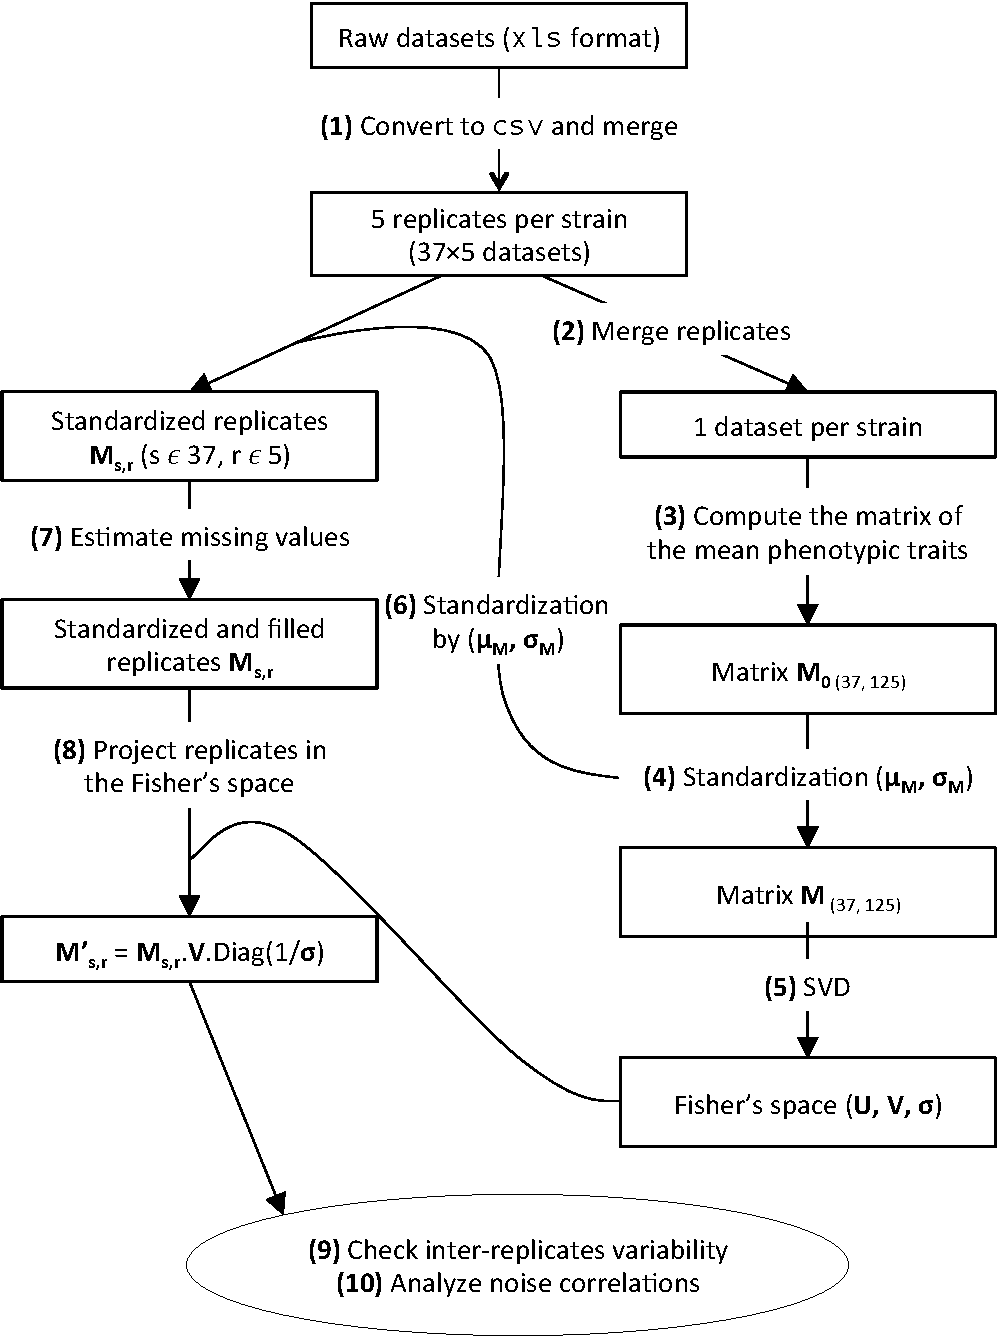
\includegraphics[scale=0.75]{part1_appendixS1_fig1.pdf}
\end{adjustwidth}
\caption[Step-by-step protocol used to analyze single-cell data.]{
\textbf{Step-by-step protocol used to analyze single-cell data.}
\textbf{(1)} Each \texttt{xls} file is converted into \texttt{csv} format, the three files related to each replicate being merged to obtain a single dataset $\boldsymbol{M_{0,s,r}}$ ($s \in \{1,...,m=37\}$, $r \in \{1,...,5\}$) per replicate.
\textbf{(2)} The 5 replicates of each strain are merged to obtain a single dataset per strain.
\textbf{(3)} The matrix $\boldsymbol{M_0}$ of the mean phenotypic trait values per strain is computed.
\textbf{(4,6)} Datasets are standardized according to the mean vector $\boldsymbol{\mu_M} \in \mathbb{R}^{125}$ and the standard deviation vector $\boldsymbol{\sigma_M} \in \mathbb{R}^{125}$ of $\boldsymbol{M_0}$.
\textbf{(5)} A singular values decomposition (SVD) is computed from standardized inter-strain dataset $\boldsymbol{M}$ (see above for the details of the SVD).
\textbf{(7)} Replicate missing values are estimated (see above).
\textbf{(8)} Each replicate dataset is projected into Fisher's space.
\textbf{(9)} Inter-replicate variability is evaluated to ensure that experimental variability is low enough.
\textbf{(10)} Intra-strain phenotypic noise correlations are analyzed.
}
\label{part1:appendixS1:fig1}
\end{figurehere}

%%%%%%%%%%%%%%%%%%%%%%%%%%%%

\newpage

\begin{figurehere}
\begin{adjustwidth}{-0in}{0in}
\centering
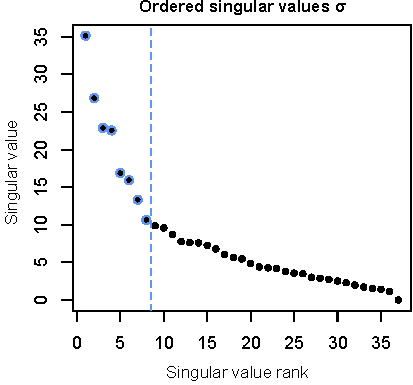
\includegraphics[scale=1.5]{part1_appendixS1_fig2.pdf}
\end{adjustwidth}
\caption[Ordered singular values contained in $\boldsymbol{\sigma}$.]{
\textbf{Ordered singular values contained in $\boldsymbol{\sigma}$.}
A simple empirical method to keep only significant variations is to isolate all the singular values located before the shoulder point in the ordered plot (as shown by a blue dashed line). Here, we kept the first 8 singular values.
}
\label{part1:appendixS1:fig2}
\end{figurehere}

%%%%%%%%%%%%%%%%%%%%%%%%%%%%

\newpage

\begin{figurehere}
\begin{adjustwidth}{-0in}{0in}
\centering
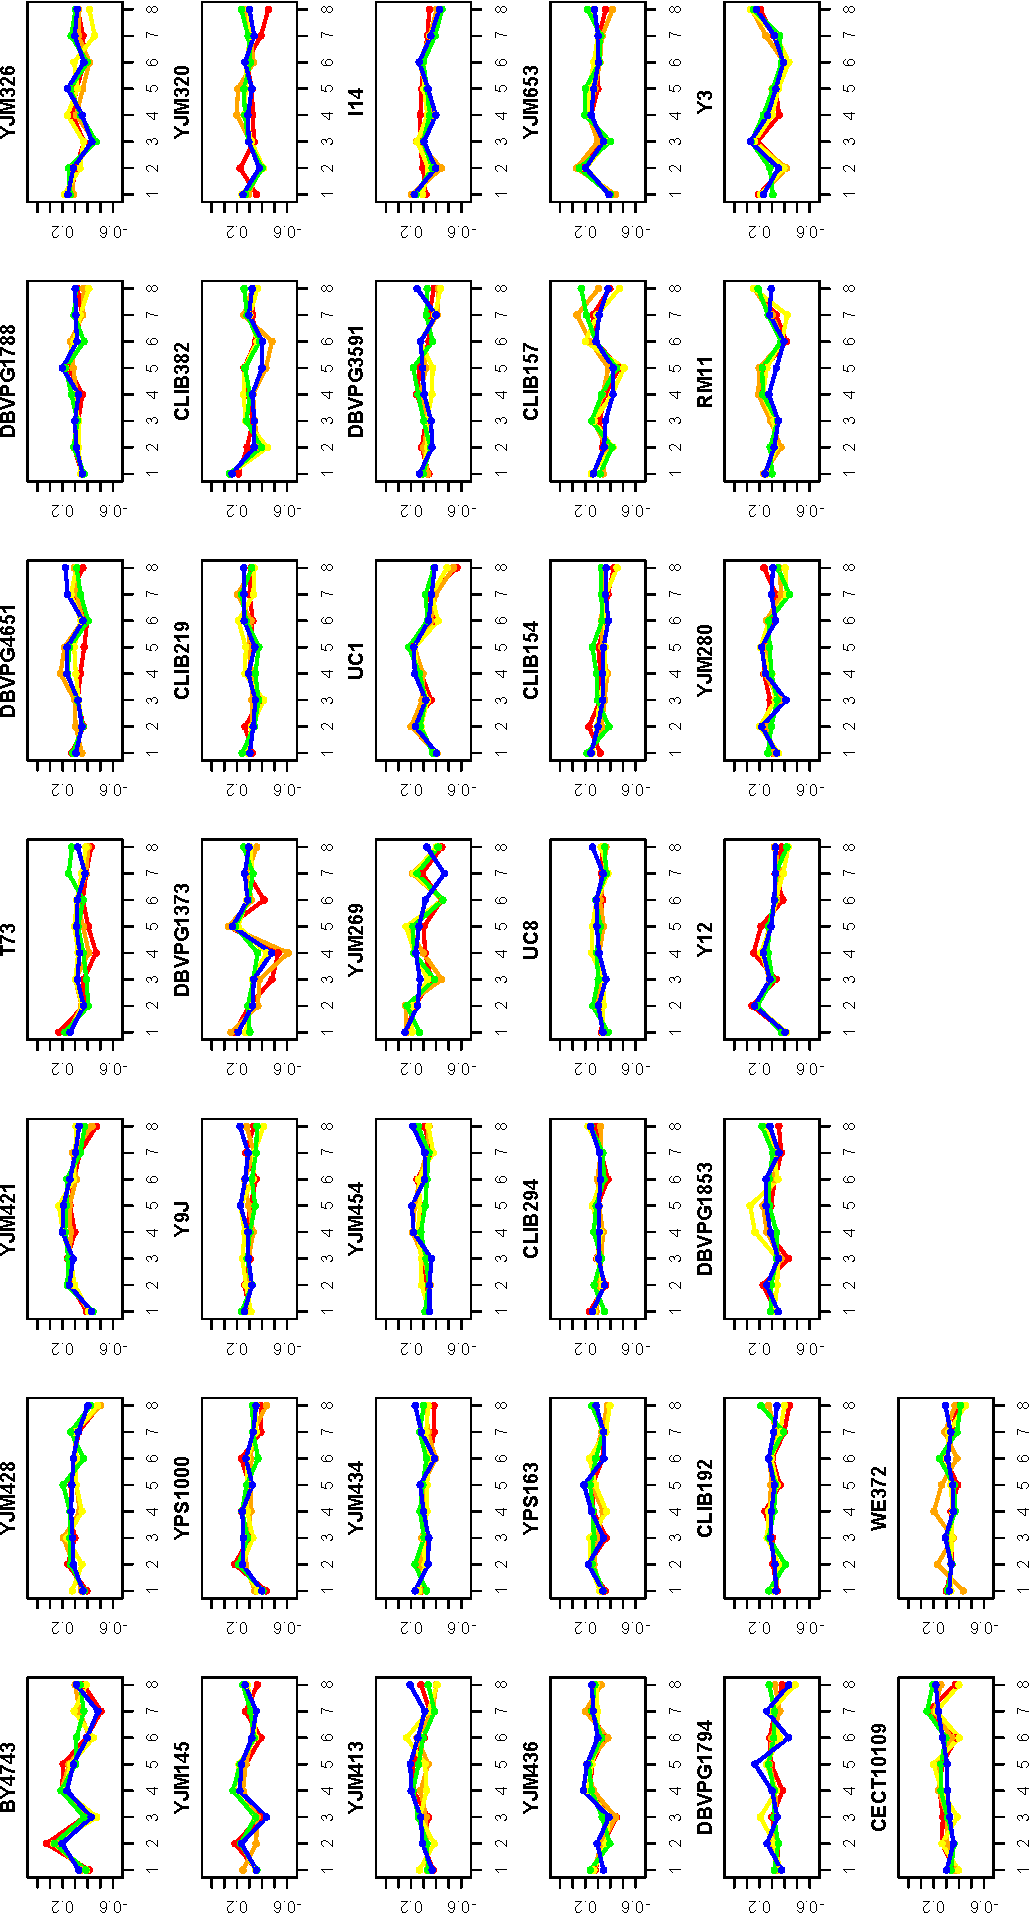
\includegraphics[scale=0.65]{part1_appendixS1_fig3.pdf}
\end{adjustwidth}
\caption[Mean phenotypic trait values per replicate per strain.]{
\textbf{Mean phenotypic trait values per replicate per strain.}
For each replicate of each strain, the mean phenotypic trait values are plotted (one color per replicate on each plot, one plot per strain).
}
\label{part1:appendixS1:fig3}
\end{figurehere}

%%%%%%%%%%%%%%%%%%%%%%%%%%%%

\newpage

\begin{figurehere}
\begin{adjustwidth}{-0in}{0in}
\centering
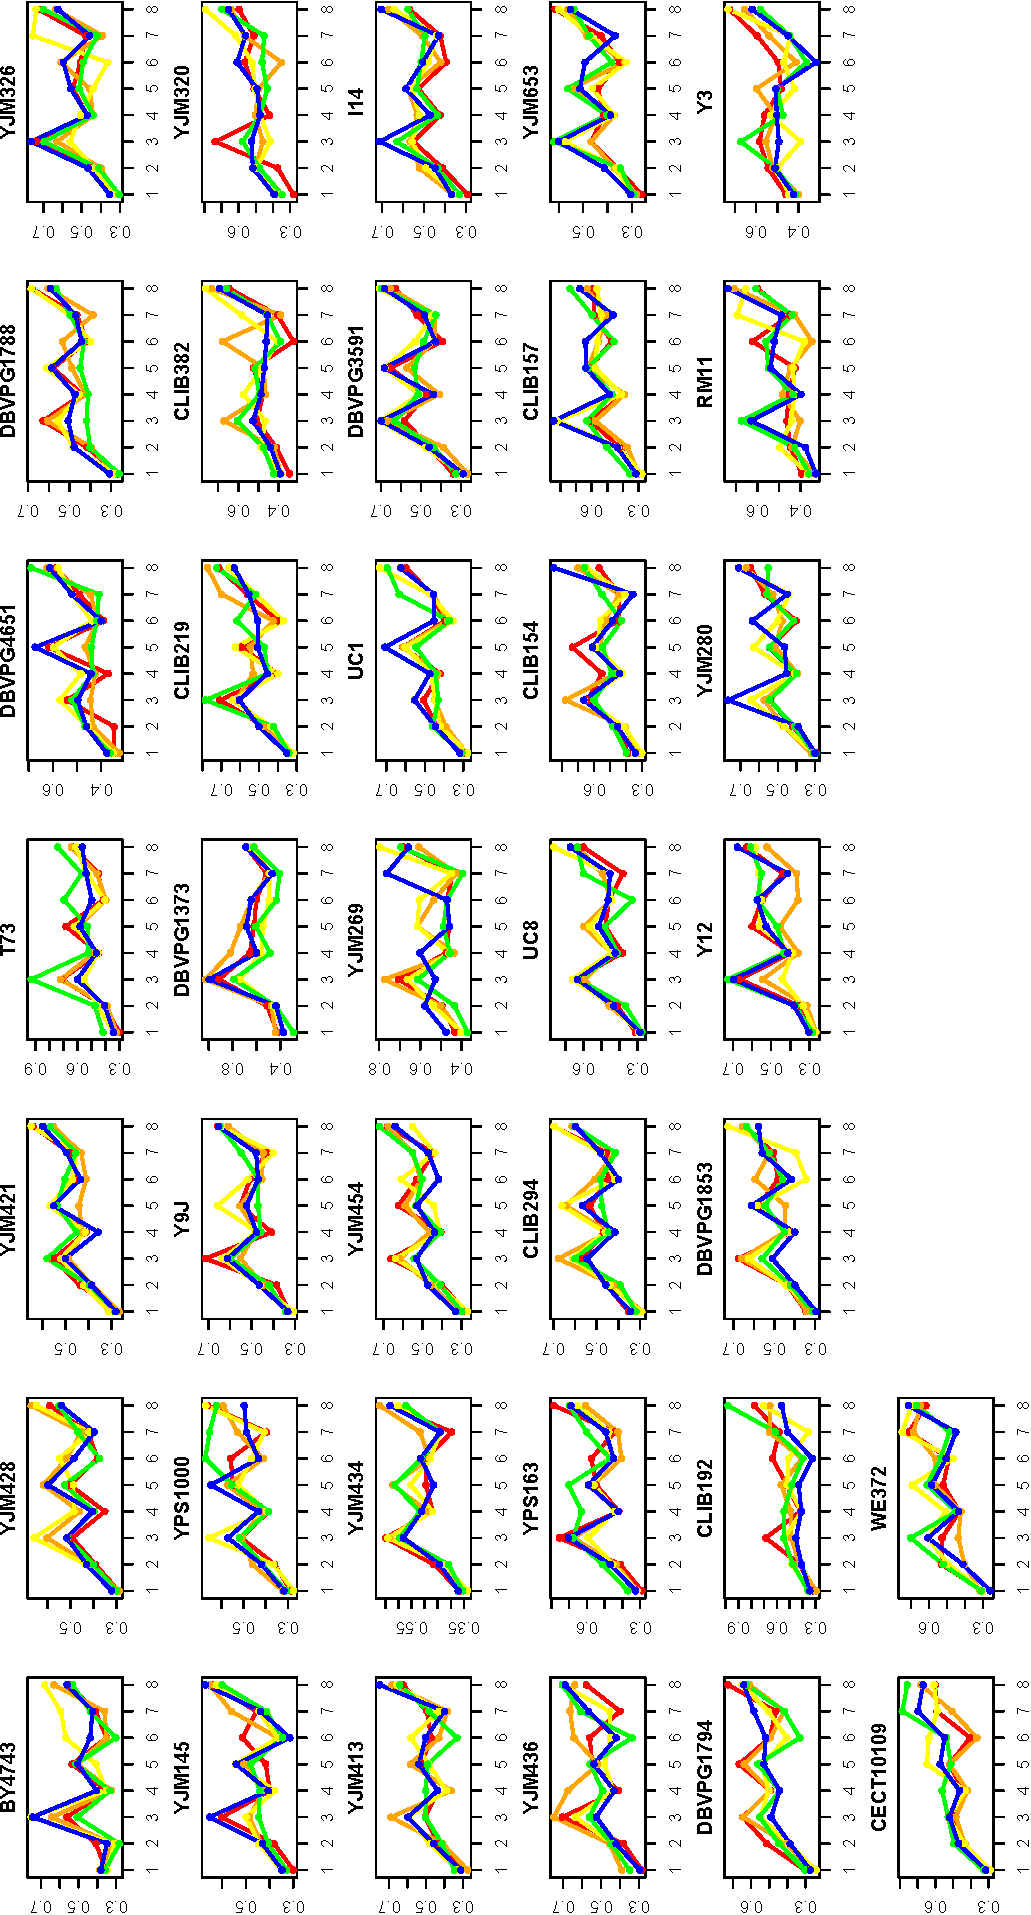
\includegraphics[scale=0.65]{part1_appendixS1_fig4.pdf}
\end{adjustwidth}
\caption[Standard deviation of each phenotypic character per replicate per strain.]{
\textbf{Standard deviation of each phenotypic character per replicate per strain.}
For each replicate of each strain, the standard deviation of each phenotypic character is plotted (one color per replicate on each plot, one plot per strain).
}
\label{part1:appendixS1:fig4}
\end{figurehere}

%%%%%%%%%%%%%%%%%%%%%%%%%%%%

\newpage

\begin{figurehere}
\begin{adjustwidth}{-0in}{0in}
\centering
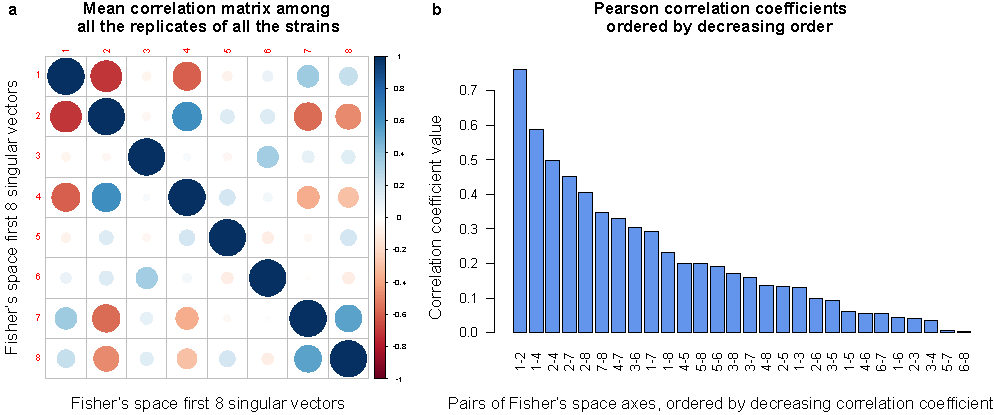
\includegraphics[scale=0.9]{part1_appendixS1_fig5.pdf}
\end{adjustwidth}
\caption[Mean phenotypic noise correlations in the Fisher's space.]{
\textbf{Mean phenotypic noise correlations in the Fisher's space.}
\textbf{a,} The mean correlation matrix across all the replicates of all the strains has been computed and plotted here. For each pair of characters, the strength of the correlation is symbolized by the size of the corresponding circle. A blue color indicates a positive correlation, and a red color a negative correlation.
\textbf{b,} All off-diagonal pairwise correlations between the first 8 axes of Fisher's space are sorted by decreasing order. The most correlated axes in mean are axes 1 and 2 (called PC1 and PC2).
}
\label{part1:appendixS1:fig5}
\end{figurehere}

%%%%%%%%%%%%%%%%%%%%%%%%%%%%

\newpage

\begin{figurehere}
\begin{adjustwidth}{-0in}{0in}
\centering
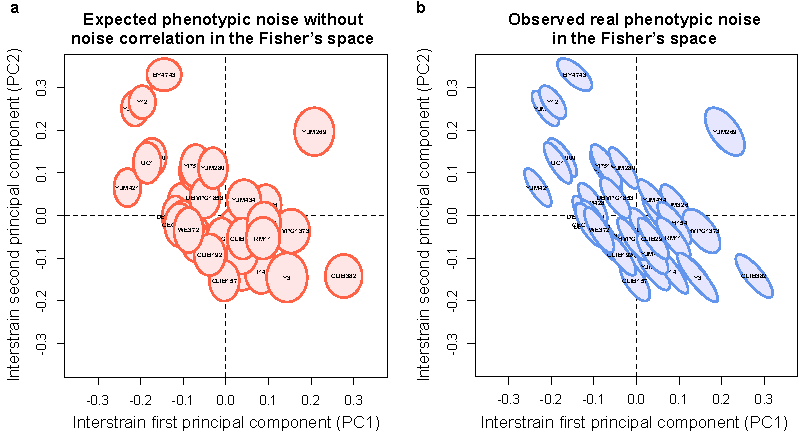
\includegraphics[scale=1]{part1_appendixS1_fig6.pdf}
\end{adjustwidth}
\caption[Yeast intra-strain phenotypic noise is correlated in the Fisher's space.]{
\textbf{Yeast intra-strain phenotypic noise is correlated in the Fisher's space.}
A singular value decomposition (SVD) was performed on the mean trait values of each of the 37 yeast strains. This space is similar to the phenotypic space used in Fisher's geometric model, where phenotypic characters mutate independently and with the same amplitude (\textit{i.e.} mean phenotype mutations are isotropic in this space). For this reason, we called this space ``Fisher's space''. We then projected single-cell data of each strain in this space. We identified the two axes showing the highest noise correlation in mean, for all strains: they correspond to the two first components of Fisher's space (PC1 and PC2).
\textbf{a,} Expected phenotypic noise for each strain without noise correlation between Fisher's space axes (each axis representing a linear combination of phenotypic characters). The shape of the phenotypic noise of each strain is symbolized by an ellipse representing the standard deviation of the associated bivariate normal law. Each ellipse is tagged with the corresponding strain name. The size of the ellipses are rescaled by a factor 0.002 to better distinguish them. The coordinates of the center of each ellipse correspond to the real position of the corresponding strain in Fisher's space (from real data).
\textbf{b,} Real observed phenotypic noise is represented, showing noise correlation between PC1 and PC2 axes, for all the strains.
}
\label{part1:appendixS1:fig6}
\end{figurehere}



\newpage

%%%%%%%%%%%%%%%%%%%%%%%%%%%

\subsection{Appendix S2. A numerical solver for {\sigmaFGM}.}
\label{part1:AppendixS2}


In this appendix, we present in more details the numerical solver of {\sigmaFGM}. We assume that the reader is aware of the basic definitions and equations provided in the main manuscript.

To estimate the evolution of the population distribution $n(\boldsymbol{\mu}, \boldsymbol{\sigma}, \boldsymbol{\theta})$ through time, we simulated the stochastic branching process associated to {\sigmaFGM} equations (as discussed in Methods). Once initial conditions are defined (Table \ref{part1:appendixS2:table1}), the evolutionary trajectory of $n(\boldsymbol{\mu}, \boldsymbol{\sigma}, \boldsymbol{\theta})$ is simulated through time using Algorithm \ref{part1:appendixS2:algorithm1}, which is similar to a time-adaptive tau-leaping algorithm \citep{gillespie-2007}.

%%%%%%%%%%%%%%%%%
%%%%%%%%%%%%%%%%%

\section*{Parameters of the numerical solver}

\begin{table}[!ht]
\begin{adjustwidth}{-0in}{0in}
\centering
\caption{List of parameters of the numerical solver for {\sigmaFGM}.}
\begin{tabular}{|l|c|c|}
\hline
Variable & Symbol & Domain\\
\hline
Number of particles & N & $[1, +\infty]$\\
Number of phenotypic characters (or dimensions) & n & $[1, +\infty]$\\
Initial mean phenotype vector & $\boldsymbol{\mu_0}$ & $\mathbb{R}^n$\\
Initial $\boldsymbol{\Sigma}$ eigenvalues vector & $\boldsymbol{\sigma_0}$ & $\mathbb{R}^{n}$\\
Initial $\boldsymbol{\Sigma}$ rotation angles vector & $\boldsymbol{\theta_0}$ & $\mathbb{R}^{n(n-1)/2}$\\
$\boldsymbol{\mu}$ values mutation size standard deviation & $s_\mu$ & $\geq 0$\\
$\boldsymbol{\sigma}$ values mutation size standard deviation & $s_\sigma$ & $\geq 0$\\
$\boldsymbol{\theta}$ values mutation size standard deviation & $s_\theta$ & $\geq 0$\\
\hline
\end{tabular}
\begin{flushleft}
These parameters must be set to initialize a stochastic branching process simulation.
\end{flushleft}
\label{part1:appendixS2:table1}
\end{adjustwidth}
\end{table}

%%%%%%%%%%%%%%%%%
%%%%%%%%%%%%%%%%%

\section*{Code availability}

The code of the numerical solver and parameter exploration scripts is freely available in Script \ref{part1:ScriptS1}, and is distributed under the open source GNU General Public License.

\newpage

%%%%%%%%%%%%%%%%%
%%%%%%%%%%%%%%%%%

\section*{Main algorithm of the numerical solver}

\begin{algorithm}[!ht]
\KwData{Set initial conditions (Table \ref{part1:appendixS2:table1}); Set $N$ particles with the same initial parameters $\boldsymbol{\mu_0}$, $\boldsymbol{\sigma_0}$ and $\boldsymbol{\theta_0}$.}
\KwResult{Evolution through time of the population distribution $n(\boldsymbol{\mu}, \boldsymbol{\sigma}, \boldsymbol{\theta})$.}
$t = 0$\;
$N_t = N$\;
\While{Stop criteria not reached}{
	$W_{max} = \max(W_i)$, for $i \in [0,N]$\;
	$dt = 0.1/W_{max}$\;
	\For{$i = 1\ ...\ N$}{
		\If{uniform\_draw(0,1) $ < W_i \times dt$}{
			$i'$ = Duplicate($i$)\;
			Mutate($i'$)\;
			$\boldsymbol{z_i}$ = multivariate\_normal\_draw($\boldsymbol{\mu_i},\boldsymbol{\Sigma_i}$)\;
			$W_i = W(\boldsymbol{z_i})$\;
			$N_t = N_t+1$\;
		}
	}
	$p_{death} = \max \left(0, (N_t-N)/N_t \right)$\;
	\For{$i = 1\ ...\ N$}{
		\If{uniform\_draw(0,1) $ < p_{death}$}{
			Kill($i$)\;
			$N_t = N_t-1$\;
		}
	}
	$t = t+dt$\;
	Compute\_moments()\;
	Compute\_statistics()\;
}
\caption{Main algorithm of the numerical solver of {\sigmaFGM}. This algorithm simulates the stochastic branching process associated to the equations of {\sigmaFGM}. In this algorithm, similar to a tau-leaping algorithm, the timestep $dt$ is not fixed and depends on the best organism's fitness $W_{max}$ at time $t$. This method is used to avoid long periods with no branching events (usually when population fitness is very low). Thus, the time scale is rescaled to set the proliferation rate of the best particle at 0.1: at each simulation time-step, $dt = 0.1/W_{max}$. The population size $N_t$ is also regulated by recomputing the death probability $p_{death}$ at each time-step such that $p_{death} = \max \left(0, (N_t-N)/N_t \right)$. Finally, at each time-step, the two first moments of $n(\boldsymbol{\mu}, \boldsymbol{\sigma}, \boldsymbol{\theta})$ are computed to extract the evolutionary trajectory, as well as the maximal eigenvalue, the maximal eigenvalue contribution and the maximal eigenvector correlation.}
\label{part1:appendixS2:algorithm1}
\end{algorithm}

%%%%%%%%%%%%%%%%%
%%%%%%%%%%%%%%%%%

\section*{Parametric exploration for a single phenotypic character.}

We performed a parametric exploration in the space $(\mu,\sigma)$ at a high resolution. More precisely, we computed the integrals in $\partial \overline{W}(\mu,\sigma)/\partial \sigma$ and $\partial \overline{W}(\mu,\sigma)/\partial \mu$ using the numerical method of Gauss-Kronrod adaptive integration on infinite intervals (QAGI) provided by the Gnu Scientific Library. We explored $\mu$ and $\sigma$ between 0 and 10, with a step of 0.01, thus representing the computation of $10^6$ points. We only explored $\mu \geq 0$ since the model is symmetric for $\mu < 0$ and $\mu > 0$.

We used the data to numerically find the ridge $\partial \overline{W}(\mu,\sigma)/\partial \sigma=0$, and the $\overline{W}(\mu,\sigma)$ gradient in the space $(\mu,\sigma)$.

%%%%%%%%%%%%%%%%%
%%%%%%%%%%%%%%%%%

\section*{Parametric exploration for an isotropic noise in $n$ dimensions}

We also performed a parametric exploration in the space $(\boldsymbol{\mu},\sigma)$ at a high resolution. We computed the integral $\partial \overline{W}(\boldsymbol{\mu},\sigma)/\partial \sigma$ using the numerical method of Gauss-Kronrod adaptive integration on infinite intervals (QAGI) provided by the Gnu Scientific Library.

We explored $\mu_1$ (all other $\mu_i, i \in \{2,\dots,n\}$ being equal to 0) and $\sigma$ between 0 and 10, with a step of 0.05, from $n=1$ to $n=50$, thus representing the computation of $2.10^6$ points. We only explored $\mu_1 \geq 0$ since the model is symmetric for $\mu_1 < 0$ and $\mu_1 > 0$.

We used the data to find numerically the ridge $\partial \overline{W}(\boldsymbol{\mu},\sigma)/\partial \sigma=0$ for each dimension, and the $\overline{W}(\boldsymbol{\mu},\sigma)$ gradient in the space $(\boldsymbol{\mu},\sigma)$.



\newpage

%%%%%%%%%%%%%%%%%%%%%%%%%%%

\subsection{Appendix S3. Analytical study of {\sigmaFGM}.}
\label{part1:AppendixS3}


In this appendix, we present in details our analytical study of {\sigmaFGM}. We assume that the reader is aware of the basic definitions and equations provided in the main manuscript.

%%%%%%%%%%%%%%%%%
%%%%%%%%%%%%%%%%%

\section*{Analytical study for a single phenotypic character}

In the single-character's version of {\sigmaFGM} ($n=1$), each organism owns two evolvable parameters $\mu \in \mathbb{R}$ and $\sigma \in \mathbb{R}_+$, encoding for the phenotypic distribution $z \sim \mathcal{N}(\mu,\sigma^2)$. The probability density to express the phenotype $z$ is:
\begin{equation}
p(z,\mu,\sigma) = \dfrac{1}{\sigma \sqrt{2\pi}} \exp \left[ \dfrac{-(z-\mu)^2}{2\sigma^2} \right].
\end{equation}
The fitness $W(z)$ of the expressed phenotype $z$ reads:
\begin{equation}
W(z) = \exp \left[ -z^2/2 \right].
\end{equation}
However, it is much more informative to look at the expected fitness $\overline{W}(\mu,\sigma)$ of an organism $(\mu,\sigma)$, that reads:
\begin{equation}
\begin{array}{rcl}
\overline{W}(\mu,\sigma) & = & \displaystyle\int_z p(z,\mu,\sigma)W(z)dz\\\\
& = & \displaystyle\int_z \dfrac{1}{\sigma \sqrt{2\pi}} \exp \left[ \dfrac{-(z-\mu)^2}{2\sigma^2} \right] \exp \left[ -\dfrac{z^2}{2} \right] dz.
\end{array}
\label{eq:part1:mean_fitness}
\end{equation}
We performed an analytical study of $\overline{W}(\mu,\sigma)$ in the space $(\mu,\sigma)$. We computed the partial derivatives $\partial \overline{W}(\mu,\sigma)/\partial \mu$ and $\partial \overline{W}(\mu,\sigma)/\partial \sigma$ in order to predict what would be the selective pressures on $\mu$ and $\sigma$, depending on the distance from the fitness optimum $z_{opt} = 0$. 

By way of introduction, we know that for $f$ continuously differentiable in $x$ and $t$, according to the Leibniz's rule:
\begin{equation}
\dfrac{d}{dt} \int_{\mathbb{R}} f(x,t)dx = \int_{\mathbb{R}} \dfrac{\partial}{\partial t} f(x,t) dx.
\label{eq:part1:leibniz_rule}
\end{equation}
Let us define the function $f(z,\mu,\sigma)$ such that:
\begin{equation}
f(z,\mu,\sigma) = p(z,\mu,\sigma)W(z)
\label{eq:part1:f_function}
\end{equation}

then:
\begin{equation}
\overline{W}(\mu,\sigma) = \displaystyle\int_{\mathbb{R}} f(z,\mu,\sigma)dz.
\label{eq:part1:int_f}
\end{equation}

%%%%%%%%%%%%%%%%%

\subsection*{Partial derivation on $\mu$}

According to Equations \ref{eq:part1:leibniz_rule} and \ref{eq:part1:int_f}, we know that:
\begin{equation}
\begin{array}{rcl}
\dfrac{\partial \overline{W}(\mu,\sigma)}{\partial \mu} & = & \displaystyle\int_z \dfrac{\partial}{\partial \mu} f(z,\mu,\sigma) dz.
\end{array}
\end{equation}

Let us compute $\partial f / \partial \mu$:

\begin{equation}
\begin{array}{rcl}
\dfrac{\partial f}{\partial \mu} & = & \dfrac{1}{\sigma \sqrt{2\pi}} \exp \left[ -\dfrac{z^2}{2} \right] \left(\exp \left[ \dfrac{-(z-\mu)^2}{2\sigma^2} \right] \right)'\\\\
& = & \dfrac{1}{\sigma \sqrt{2\pi}} \exp \left[ -\dfrac{z^2}{2} \right] \dfrac{(z-\mu)}{\sigma^2} \exp \left[ \dfrac{-(z-\mu)^2}{2\sigma^2} \right]\\\\
& = & \dfrac{(z-\mu)}{\sigma^2} f(z,\mu,\sigma)\\\\
& = & \dfrac{(z-\mu)}{\sigma^2} p(z,\mu,\sigma)W(z)
\end{array}
\label{eq:part1:mu_derivation}
\end{equation}

$p(z,\mu,\sigma)$ being a Gaussian density, we know that:
\begin{equation}
\dfrac{\partial p(z,\mu,\sigma)}{\partial z} = -\dfrac{(z-\mu)}{\sigma^2}\ p(z,\mu,\sigma).
\end{equation}

Then, Equation \ref{eq:part1:mu_derivation} can be rewritten as following:
\begin{equation}
\dfrac{\partial f(z,\mu,\sigma)}{\partial \mu} = -\dfrac{\partial p(z,\mu,\sigma)}{\partial z}W(z).
\end{equation}

Here, the goal here is to determine the sign of $\partial \overline{W}(\mu,\sigma)/\partial \mu$, that reads:
\begin{equation}
\begin{array}{rcl}
\dfrac{\partial \overline{W}(\mu,\sigma)}{\partial \mu} & = & \displaystyle\int_z \dfrac{\partial f(z,\mu,\sigma)}{\partial \mu} dz\\\\
& = & \displaystyle\int_z \underbrace{-\dfrac{\partial p(z,\mu,\sigma)}{\partial z}}_{\text{Anti-symmetric function}} \times \underbrace{W(z)}_{\text{Symmetric function}} dz.
\end{array}
\label{eq:part1:mu_full_equation}
\end{equation}

To determine the sign of $\partial \overline{W}(\mu,\sigma)/\partial \mu$, we must consider the shape of the integrated function, being the product of:
\begin{enumerate}
\item[\textbf{(1)}] $-\partial p(z,\mu,\sigma)/\partial z$, an anti-symmetric function centered on $\mu$, negative if $z < \mu$, and positive if $z > \mu$ (Fig. \ref{part1:appendixS3:fig1}a);
\item[\textbf{(2)}] $W(z)$, a strictly positive and symmetric function, centered on 0  (Fig. \ref{part1:appendixS3:fig1}b).
\end{enumerate}

When $\mu=0$, the product of the anti-symmetric and symmetric functions $\partial p(z,\mu,\sigma)/\partial z \times W(z)$ is an anti-symmetric function, its integral thus being equal to zero (Figs. \ref{part1:appendixS3:fig1}c and \ref{part1:appendixS3:fig1}d). Then, the sign of $\partial \overline{W}(\mu,\sigma)/\partial \mu$ depends on $\mu$ as following:
\begin{equation}
\left\{
\begin{array}{rcl}
\text{If } \mu < 0 &,& \partial f(z,\mu,\sigma)/\partial \mu > 0\\\\
\text{If } \mu = 0 &,& \partial f(z,\mu,\sigma)/\partial \mu = 0\\\\
\text{If } \mu > 0 &,& \partial f(z,\mu,\sigma)/\partial \mu < 0
\end{array}
\right.
\end{equation}

Hence, for any value of $\sigma > 0$, the selective pressures act to reduce $\mu$ towards $\mu=0$, defining a ridge $\partial \overline{W}(\mu,\sigma)/\partial \mu = 0$ when $\mu = 0$. Any organism owning a value of $\mu \neq 0$ has a lower fitness than an organism with $\mu = 0$, for any given value of $\sigma$. This ridge is plotted in purple on Figure \ref{part1:appendixS3:fig3}.

As revealed in Equation \ref{eq:part1:mu_derivation}, two other conditions exist for $\partial W(\mu,\sigma)/\partial \mu = 0$:
\begin{equation}
\left\{
\begin{array}{rcl}
\text{If } \mu \rightarrow \pm \infty &,& \partial f(z,\mu,\sigma)/\partial \mu = 0\\\\
\text{If } \sigma \rightarrow +\infty &,& \partial f(z,\mu,\sigma)/\partial \mu = 0\\\\
\end{array}
\right.
\end{equation}

Thus, organisms located very far from the fitness optimum (\textit{i.e.}, $|\mu| \gg 0$), or organisms with a very dispersed phenotypic distribution (\textit{i.e.}, $\sigma \gg 0$), do not experience selective pressures. However, according to Equation \ref{eq:part1:mean_fitness}, their mean fitness $\overline{W}(\mu, \sigma)$ is almost equal to zero in these conditions.

Another critical condition to clarify for the partial derivative $\partial \overline{W}(\mu,\sigma)/\partial \mu$ is when $\sigma \rightarrow 0$. Equation \ref{eq:part1:mu_full_equation} can help us to solve this special case. Indeed, normal distributions with parameters $\mu$ and $\sigma$ converge towards a Dirac distribution $\delta(z-\mu)$ when $\sigma \rightarrow 0$. The Dirac distribution satisfies, for all continuous function $\varphi(z)$,
\begin{equation}
\int_z \delta(z-\mu)\varphi(z)dz = \varphi(\mu).
\end{equation}

The first derivative of the Dirac distribution (in the sense of distributions) satisfies:
\begin{equation}
\displaystyle\int_{\mathbb{R}} \delta'(z-\mu)\varphi(z)dz = -\varphi'(\mu)
\end{equation}
and the $n$-th derivative, denoted $\delta^{(n)}$, satisfies:
\begin{equation}
\displaystyle\int_z \delta^{(n)}(z-\mu) \varphi(z) dz = (-1)^n \varphi^{(n)}(\mu).
\end{equation}
 
Thus, starting from Equation \ref{eq:part1:mu_full_equation}, we can derive the following limiting equation when $\sigma \rightarrow 0$:
\begin{equation}
\begin{array}{rcl}
\lim\limits_{\sigma \to 0}\ \dfrac{\partial \overline{W}}{\partial \mu} & = & \lim\limits_{\sigma \to 0}\ \dfrac{\partial}{\partial \mu} \displaystyle\int_{\mathbb{R}} p(z,\mu,\sigma)W(z)dz\\\\
& = & \dfrac{\partial}{\partial \mu} \lim\limits_{\sigma \to 0}\ \displaystyle\int_{\mathbb{R}} p(z,\mu,\sigma)W(z)dz\\\\
& = & \dfrac{\partial}{\partial \mu} \displaystyle\int_{\mathbb{R}} \delta(z-\mu)W(z)dz\\\\
& = & \dfrac{\partial W(\mu)}{\partial \mu}\\\\
& = & W'(\mu).
\end{array}
\label{eq:part1:sigma_zero_limit}
\end{equation}

Thus, when $\sigma \rightarrow 0$, the system converges towards canonical FGM scenario, according that $\mu \equiv z$ in this case.

%%%%%%%%%%%%%%%%%

\subsection*{Partial derivation on $\sigma$}

We first rewrite the equation $f(z,\mu,\sigma)$ to separate $\sigma$ from other terms:
\begin{equation}
f(z,\mu,\sigma) = \dfrac{W(z)}{\sqrt{2\pi}} \times \dfrac{1}{\sigma} \exp \left[\dfrac{-(z-\mu)^2}{2\sigma^2}\right].
\end{equation}
Let us define the term $a = W(z)/\sqrt{2\pi}$ that does not depend on $\sigma$, such that:
\begin{equation}
f(z,\mu,\sigma) = a \times \dfrac{1}{\sigma} \exp \left[\dfrac{-(z-\mu)^2}{2\sigma^2}\right].
\end{equation}

The partial derivation of $f$ with respect to $\sigma$ is more technical than for $\mu$. We describe it step by step below.
Let us define the terms $u$ and $v$ such that:
\begin{equation}
\left\{
\begin{array}{rcl}
u & = & \exp \left[\dfrac{-(z-\mu)^2}{2\sigma^2} \right]\\\\
v & = & \sigma
\end{array}
\right.
\end{equation}
Then:
\begin{equation}
\dfrac{\partial f(z,\mu,\sigma)}{\partial \sigma} = a \times \dfrac{(u'v-uv')}{v^2}
\end{equation}
with:
\begin{equation}
\left\{
\begin{array}{rcl}
u' & = & \dfrac{(z-\mu)^2}{\sigma^3} \exp \left[\dfrac{-(z-\mu)^2}{2\sigma^2} \right]\\\\
v' & = & 1
\end{array}
\right.
\end{equation}

Thus, the derivative $\partial f/\partial \sigma$ reads:
\begin{equation}
\begin{array}{rcl}
\dfrac{\partial f(z,\mu,\sigma)}{\partial \sigma} & = & a \times \left( \dfrac{\dfrac{\sigma(z-\mu)^2}{\sigma^3} \exp \left[\dfrac{-(z-\mu)^2}{2\sigma^2}\right] - \exp \left[\dfrac{-(z-\mu)^2}{2\sigma^2}\right]}{\sigma^2}\right)\\\\
& = & a \times \exp \left[\dfrac{-(z-\mu)^2}{2\sigma^2}\right] \times \left( \dfrac{\dfrac{(z-\mu)^2}{\sigma^2} - 1}{\sigma^2}\right)\\\\
& = & a \times \exp \left[\dfrac{-(z-\mu)^2}{2\sigma^2}\right] \times \dfrac{(z-\mu)^2-\sigma^2}{\sigma^4}\\\\
& = & \dfrac{(z-\mu)^2-\sigma^2}{\sigma^3}\ f(z,\mu,\sigma)\\\\
& = & \dfrac{(z-\mu)^2-\sigma^2}{\sigma^3}\ p(z,\mu,\sigma)W(z)\\\\
\end{array}
\label{eq:part1:sigma_derivative}
\end{equation}

$p(z)$ being the density of a normal law, we know that:
\begin{equation}
\dfrac{\partial^2 p(z,\mu,\sigma)}{\partial z^2} = \dfrac{(z-\mu)^2-\sigma^2}{\sigma^4}\ p(z,\mu,\sigma).
\end{equation}

From Equation \ref{eq:part1:sigma_derivative}, we thus find:
\begin{equation}
\dfrac{\partial f(z,\mu,\sigma)}{\partial \sigma} = \underbrace{\dfrac{\partial^2 p(z,\mu,\sigma)}{\partial z^2}}_{\text{Symmetric function}} \times \underbrace{\sigma\ W(z)}_{\text{Symmetric function}}.
\end{equation}

We were not able to compute the ridge $\partial \overline{W}(\mu,\sigma)/\partial \sigma=0$. We used a numerical scheme to compute $\partial \overline{W}(\mu,\sigma)/\partial \sigma$ depending on $\mu$ and $\sigma$ (see Appendix \ref{part1:AppendixS2}).

However, it is possible to determine analytically some essential characteristics of the ridge $\partial \overline{W}(\mu,\sigma)/\partial \sigma=0$ (Fig. \ref{part1:appendixS3:fig3} orange curve):
\begin{enumerate}
\item[\textbf{(1)}] The sign of $\partial \overline{W}(\mu,\sigma)/\partial \sigma$ when $\sigma \rightarrow 0$;
\item[\textbf{(2)}] The position of the inflection point $\mu=d_{th}$, below which the phenotypic noise is always deleterious (Fig. \ref{part1:appendixS3:fig3} orange circle).
\end{enumerate}

\paragraph{(1)}
As previously (Eq. \ref{eq:part1:sigma_zero_limit}), when $\sigma \rightarrow 0$, $\partial \overline{W}(\mu,\sigma)/\partial \sigma$ reads:
\begin{equation}
\begin{array}{rcl}
\lim\limits_{x \to 0}\ \dfrac{\partial \overline{W}(\mu,\sigma)}{\partial \sigma} & = & \displaystyle\int_z \delta^{''}(z-\mu) \times \sigma\ W(z) dz\\\\
& = & (-1)^2 \sigma\ W^{''}(\mu)\\\\
& = & \sigma (\mu^2-1) \ W(\mu)\\\\
& = & 0.
\end{array}
\end{equation}

Thus, when $\sigma \rightarrow 0$, the first order selective pressure on $\sigma$ vanishes, for any values of $\mu$. This means that to determine whether low noise levels are beneficial, one must look at the second derivative of $\overline{W}$ with respect to $\sigma$, and identify the inflection points that separate the regions where noise is beneficial or deleterious.

\paragraph{(2)}

We first compute $\partial^2 f/\partial \sigma^2$. From Equation \ref{eq:part1:sigma_derivative}, we define the terms $u$ and $v$ such that:
\begin{equation}
\left\{
\begin{array}{rcl}
u & = & \dfrac{(z-\mu)^2-\sigma^2}{\sigma^3}\\\\
v & = & f(z,\mu,\sigma)
\end{array}
\right.
\end{equation}

Thus, $\partial^2 f/\partial \sigma^2 = u'v+uv'$, with:
\begin{equation}
\begin{array}{rcl}
u' & = & \dfrac{\sigma^2-3(z-\mu)^2}{\sigma^4}\\\\
v' & = & \dfrac{(z-\mu)^2-\sigma^2}{\sigma^3} f(z,\mu,\sigma)
\end{array}
\end{equation}

%%%%%%%%%%%%%%%%%%%%%%%%%%%%%%%%%%%%%%%%%%%%
% FIGURES
%%%%%%%%%%%%%%%%%%%%%%%%%%%%%%%%%%%%%%%%%%%%

\begin{figure}[!h]
\begin{adjustwidth}{-0in}{0in}
\centering
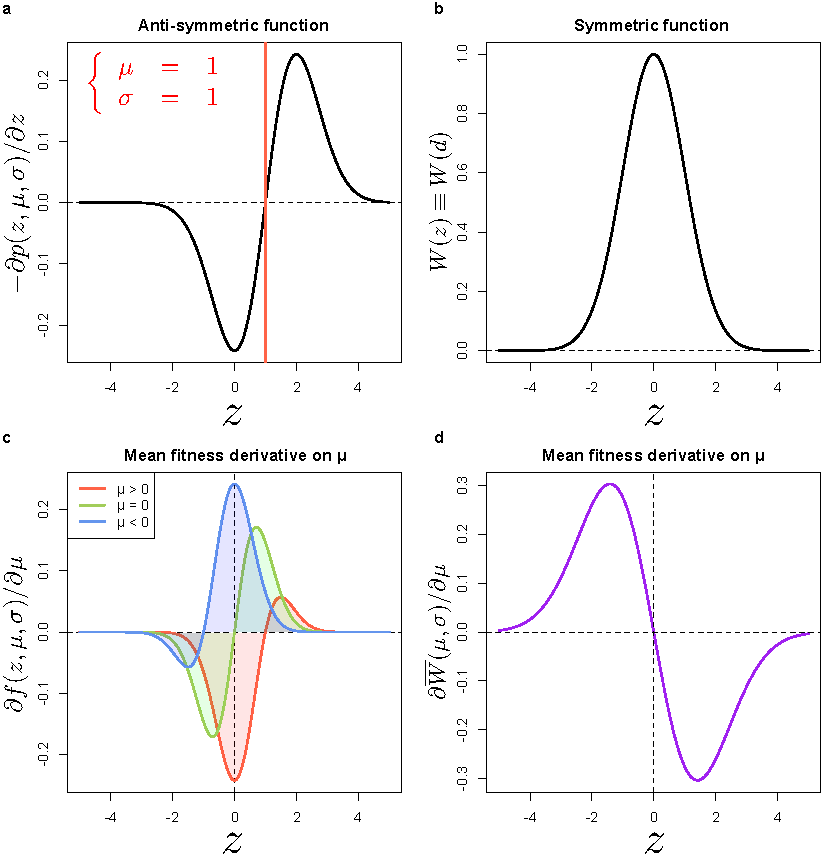
\includegraphics[scale=1]{part1_appendixS3_fig1.pdf}
\end{adjustwidth}
\caption[Behavior of $\partial \overline{W}(\mu,\sigma)/\partial \mu$.]{
\textbf{Behavior of $\partial \overline{W}(\mu,\sigma)/\partial \mu$.}
\textbf{a,} The normal distribution derivative $-\partial p(z,\mu,\sigma)/\partial z$ is an anti-symmetric function centered on $z=\mu$, such that the function is negative when $z < \mu$ and positive when $z > \mu$. Here, an example is given for $\mu=1$ and $\sigma=1$. The red vertical line represents the value of $\mu$, which is an axis of symmetry of the function.
\textbf{b,} The Gaussian-shaped fitness function $W(z)$ is a strictly positive, symmetric function centered on $z=0$.
\textbf{c,d,} The product of both functions, equal to $\partial f(z,\mu,\sigma)/\partial \mu$ is biased towards positive values if $\mu < 0$ (blue curve), towards negative values if $\mu > 0$ (red curve), or anti-symmetric if $\mu=0$ (green curve). Thus the integral $\int_z \partial f(z,\mu,\sigma)/\partial \mu\ dz$ is respectively positive, negative, or zero, if $\mu$ is negative, positive or zero (as shown in panel \textbf{d}, purple curve).
}
\label{part1:appendixS3:fig1}
\end{figure}

\begin{figure}[!h]
\begin{adjustwidth}{-0in}{0in}
\centering
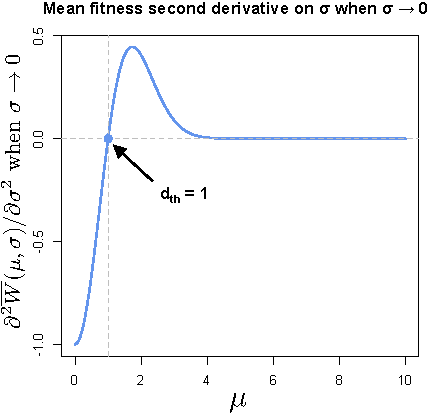
\includegraphics[scale=1]{part1_appendixS3_fig2.pdf}
\end{adjustwidth}
\caption[Variation of $\partial^2 W(\mu,\sigma)/\partial \sigma^2$ when $\sigma \rightarrow 0$.]{
\textbf{Variation of $\partial^2 \overline{W}(\mu,\sigma)/\partial \sigma^2$ when $\sigma \rightarrow 0$.}
The variation of $\partial^2 \overline{W}(\mu,\sigma)/\partial \sigma^2$ when $\sigma \rightarrow 0$ is represented here depending on $\mu$. It is described by Equation \ref{eq:part1:d2wdsigma}. Blue dot: inflection point of the ridge $\partial \overline{W}(\mu,\sigma)/\partial \sigma = 0$ (Fig. \ref{part1:appendixS3:fig3} orange circle), for $\mu = d_{th} = 1$.
}
\label{part1:appendixS3:fig2}
\end{figure}

\begin{figure}[!h]
\begin{adjustwidth}{-0in}{0in}
\centering
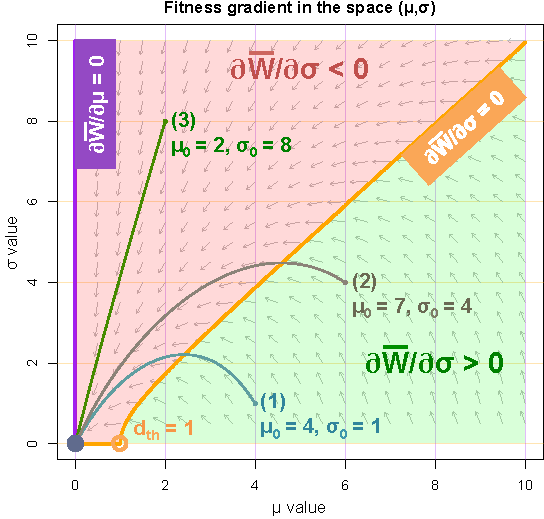
\includegraphics[scale=1]{part1_appendixS3_fig3.pdf}
\end{adjustwidth}
\caption[Variations of the mean fitness $\overline{W}(\mu,\sigma)$ in the space $(\mu,\sigma)$.]{\textbf{Variations of the mean fitness $\overline{W}(\mu,\sigma)$ in the space $(\mu,\sigma)$.}
In purple, the ridge $\partial \overline{W}/\partial \mu=0$. In orange, the ridge $\partial \overline{W}/\partial \sigma=0$. Green area: $\partial \overline{W}/\partial \sigma > 0$ (\textit{i.e.}, it is beneficial to increase the phenotypic noise). Red area: $\partial \overline{W}/\partial \sigma < 0$ (\textit{i.e.}, it is beneficial to reduce the phenotypic noise). Three trajectories following the fitness gradient are represented \textbf{(1)} in blue (initial values: $\mu_0=4, \sigma_0=1$), \textbf{(2)} in brown (initial values: $\mu_0=6, \sigma_0=4$) and \textbf{(3)} in green (initial values: $\mu_0=2, \sigma_0=8$). Black dot: fitness optimum $z_{opt}$. Orange circle: inflection point $d_{th}=1$ of the fitness landscape $W(z)$. Grey arrows indicate the direction of the fitness gradient, but not its amplitude.
}
\label{part1:appendixS3:fig3}
\end{figure}

%%%%%%%%%%%%%%%%%%%%%%%%%%%%%%%%%%%%%%%%%%%%
%%%%%%%%%%%%%%%%%%%%%%%%%%%%%%%%%%%%%%%%%%%%

The second derivative of $f$ then reads:
\begin{equation}
\begin{array}{rcl}
\dfrac{\partial^2 f(z,\mu,\sigma)}{\partial \sigma^2} & = & \dfrac{(z-\mu)^2-\sigma^2}{\sigma^3} f(z,\mu,\sigma) + \left( \dfrac{\sigma^2-3(z-\mu)^2}{\sigma^4}\right)^2 f(z,\mu,\sigma)\\\\
& = & f(z,\mu,\sigma) \left( \dfrac{\sigma^4-3\sigma^2(z-\mu)^2+(z-\mu)^4-2(z-\mu)^2\sigma^2+\sigma^4}{\sigma^6} \right)\\\\
& = & f(z,\mu,\sigma) \left( \dfrac{2\sigma^4-5(z-\mu)^2\sigma^2+(z-\mu)^4}{\sigma^6} \right).
\end{array}
\end{equation}
As demonstrated previously, it is possible to rewrite this equation to extract derivatives of normal law densities:
\begin{equation}
\begin{array}{rcl}
\dfrac{\partial^2 f(z,\mu,\sigma)}{\partial \sigma^2} & = & f(z,\mu,\sigma) \left( \dfrac{(z-\mu)^4-6(z-\mu)^2\sigma^2+3\sigma^4}{\sigma^6}+\dfrac{(z-\mu)^2\sigma^2-\sigma^4}{\sigma^6} \right)\\\\
& = & \sigma^2\ f(z,\mu,\sigma) \left( \dfrac{(z-\mu)^4-6(z-\mu)^2\sigma^2+3\sigma^4}{\sigma^8} + \dfrac{1}{\sigma^2}\dfrac{(z-\mu)^2-\sigma^2}{\sigma^4} \right)\\\\
& = & \sigma^2\ f(z,\mu,\sigma) \left( \dfrac{(z-\mu)^4-6(z-\mu)^2\sigma^2+3\sigma^4}{\sigma^8} + \dfrac{(z-\mu)^2-\sigma^2}{\sigma^6} \right)\\\\
& = & \sigma^2\ W(z) \left( \dfrac{\partial^4 p(z,\mu,\sigma)}{\partial z^4} + \dfrac{1}{\sigma^2} \times \dfrac{\partial^2 p(z,\mu,\sigma)}{\partial z^2} \right)\\\\
& = & \underbrace{\left( \sigma^2\ W(z) \dfrac{\partial^4 p(z,\mu,\sigma)}{\partial z^4} \right)}_{\rightarrow 0 \text{ when } \sigma \rightarrow 0} + \left(W(z) \dfrac{\partial^2 p(z,\mu,\sigma)}{\partial z^2} \right).
\end{array}
\label{eq:part1:second_derivative}
\end{equation}

Consequently, when $\sigma \rightarrow 0$, the partial derivative $\partial^2 \overline{W}(\mu,\sigma)/\partial \sigma^2$ reads:
\begin{equation}
\lim\limits_{x \to 0}\ \dfrac{\partial^2 \overline{W}(\mu,\sigma)}{\partial \sigma^2} = (\mu^2-1)\ W(\mu).
\label{eq:part1:d2wdsigma}
\end{equation}

The only value of $\mu$ for which $\partial^2 \overline{W}(\mu,\sigma)/\partial \sigma^2 = 0$ is $|\mu| = 1$. When $|\mu| < 1$, $\partial^2 \overline{W}(\mu,\sigma)/\partial \sigma^2 < 0$, meaning that the selective pressure is towards a reduction of the phenotypic noise $\sigma$. When $|\mu| > 1$, $\partial^2 \overline{W}(\mu,\sigma)/\partial \sigma^2 > 0$, meaning that the selective pressure is towards an increase of the phenotypic noise $\sigma$ (Fig. \ref{part1:appendixS3:fig2} blue curve, and Fig. \ref{part1:appendixS3:fig3} orange curve and circle). Thus, $d_{th}=1$.

%%%%%%%%%%%%%%%%%
%%%%%%%%%%%%%%%%%

\section*{Analytical and numerical studies of an isotropic noise on $n$ phenotypic characters}

As described in Results, an isotropic noise is applied to the mean phenotype $\boldsymbol{\mu}$, by independently varying each trait value $\mu_i$ with the same noise amplitude $\sigma$. The probability $p(\boldsymbol{z},\boldsymbol{\mu},\sigma)$ for an organism $(\boldsymbol{\mu}, \sigma)$ to express the phenotype $\boldsymbol{z}$ is then:
\begin{equation}
p(\boldsymbol{z},\boldsymbol{\mu},\sigma) = \prod_{i \in n} \dfrac{1}{\sigma \sqrt{2\pi}} \exp \left[ \dfrac{-(z_i-\mu_i)^2}{2\sigma^2} \right].
\end{equation}

As in the previous section, the goal is to compute the second derivative of $\overline{W}(\boldsymbol{\mu}, \sigma)$ on $\sigma$, and find its inflection point to detect the critical euclidean distance $d_{th}$ below which phenotypic noise must be minimized. However, we now must compute it in $n$ dimensions. Hopefully, two conditions allow us to strongly simplify the equations:
\begin{enumerate}
\item[\textbf{(1)}] Noise is isotropic, such that $\overline{W}(\boldsymbol{\mu}, \sigma)$ can be decomposed in a product of one-dimensional integrals;
\item[\textbf{(2)}] The mean phenotype of an organism $\boldsymbol{\mu}$ is taken away from the fitness optimum on a single axis, all other axes remaining at a distance zero of the fitness optimum. By rotational symmetry, we can generalize to any position $\boldsymbol{\mu}$ away from the fitness optimum.
\end{enumerate}

$\overline{W}(\boldsymbol{\mu}, \sigma)$ reads:
\begin{equation}
\begin{array}{rcl}
\overline{W}(\boldsymbol{\mu}, \sigma) & = & \displaystyle\int_{\mathbb{R}^n} p(\boldsymbol{z},\boldsymbol{\mu},\sigma)W(\boldsymbol{z})d\boldsymbol{z}\\\\
& = & \displaystyle\int_{\mathbb{R}} p(z_1,\mu_1,\sigma)W(z_1)dz_1 \times ... \times \displaystyle\int_{\mathbb{R}} p(z_n,\mu_n,\sigma)W(z_n)dz_n.
\end{array}
\end{equation}

If we only move the mean phenotypic trait value $\mu_1$ away from the fitness optimum, all other mean trait values being equal to zero, $\overline{W}(\boldsymbol{\mu}, \sigma)$ then reads:
\begin{equation}
\begin{array}{rcl}
\overline{W}(\boldsymbol{\mu}, \sigma) & = & \displaystyle\int_{\mathbb{R}} p(z_1,\mu_1,\sigma)W(z_1)dz_1 \times \left( \displaystyle\int_{\mathbb{R}} p(z,0,\sigma)W(z)dz \right)^{n-1}.
\end{array}
\end{equation}

As demonstrated above, we know that for a single character and when $\sigma \rightarrow 0$, the successive derivatives of $\overline{W}(\mu, \sigma)$ read:
\begin{equation}
\left\{
\begin{array}{ccl}
\overline{W} & = & W(\mu)\\\\
\overline{W}' & = & 0\\\\
\overline{W}'' & = & (\mu^2-1)W(\mu)
\end{array}
\right.
\label{eq:part1:derivative1}
\end{equation}

Moreover, when $\mu = 0$, we find that:
\begin{equation}
\left\{
\begin{array}{ccl}
\overline{W}_0 & = & 1\\\\
\overline{W}_0' & = & 0\\\\
\overline{W}_0'' & = & -1
\end{array}
\right.
\label{eq:part1:derivative2}
\end{equation}

We then define the terms $a$, $b$ and $c$ such that:
\begin{equation}
\left\{
\begin{array}{ccl}
a & = & \displaystyle\int_{\mathbb{R}} p(z_1,\mu_1,\sigma)W(z_1)dz_1\\\\
b & = & \displaystyle\int_{\mathbb{R}} p(z,0,\sigma)W(z)dz\\\\
c & = & b^{\ n-1}
\end{array}
\right.
\end{equation}

We now compute the second derivative of $\overline{W}(\boldsymbol{\mu}, \sigma)$ on $\sigma$, according to $a$, $b$ and $c$, this equation reads:
\begin{equation}
\dfrac{\partial^2 \overline{W}(\boldsymbol{\mu}, \sigma)}{\partial \sigma^2} = ac'' + 2a'c' + a''c
\end{equation}
With:
\begin{equation}
\left\{
\begin{array}{ccl}
c' & = & (n-1)b'b^{\ n-2}\\\\
c'' & = & (n-1)(n-2)b'b^{\ n-3} + (n-1)b''b^{\ n-2}
\end{array}
\right.
\end{equation}

Then, the complete equation of $\partial \overline{W}(\boldsymbol{\mu}, \sigma) / \partial \sigma$ reads:
\begin{equation}
\begin{array}{rcl}
\dfrac{\partial^2 \overline{W}(\boldsymbol{\mu}, \sigma)}{\partial \sigma^2} & = & a \left( (n-1)(n-2)b'b^{\ n-3} + (n-1)b''b^{\ n-2} \right)\\\\
& + & 2a'(n-1)b'b^{\ n-2}\\\\
& + & a''b^{\ n-1}.
\end{array}
\end{equation}

We now replace the terms $a$ and $b$ by the corresponding terms in Equations \ref{eq:part1:derivative1} and \ref{eq:part1:derivative2}:

\begin{equation}
\begin{array}{rcl}
\dfrac{\partial^2 \overline{W}(\boldsymbol{\mu}, \sigma)}{\partial \sigma^2} & = & \overline{W} \left( (n-1)(n-2)\overline{W}_0'\overline{W}_0^{\ n-3} + (n-1)\overline{W}_0''\overline{W}_0^{\ n-2} \right)\\\\
& + & 2\overline{W}'(n-1)\overline{W}_0'\overline{W}_0^{\ n-2}\\\\
& + & \overline{W}''\overline{W}_0^{\ n-1}.
\end{array}
\end{equation}

Finally, the second derivative of $\overline{W}(\boldsymbol{\mu}, \sigma)$ on $\sigma$ reads:
\begin{equation}
\dfrac{\partial^2 \overline{W}(\boldsymbol{\mu}, \sigma)}{\partial \sigma^2} = (\mu_1^2-n)W(\mu_1).
\label{eq:part1:super_equation}
\end{equation}

The only value of $\mu_1$ for which Equation \ref{eq:part1:super_equation} is equal to zero is $\mu_1 = \pm \sqrt{n}$. Since this result is valid when the euclidean distance $d = \lVert \boldsymbol{\mu} \rVert$ is equal to $\sqrt{n}$, we can conclude that the critical distance below which isotropic phenotypic noise must be minimized is $d_{th} = \sqrt{n}$.

%%%%%%%%%%%%%%%%%
%%%%%%%%%%%%%%%%%

\section*{Anisotropic and correlated phenotypic noise is beneficial when aligned with the fitness optimum}

Let us consider the organism $(\boldsymbol{\mu}, \boldsymbol{\sigma}, \boldsymbol{\theta})$ in a $n$-dimensional phenotypic space, sitting at a certain distance of the fitness optimum $\boldsymbol{z_{opt}}$ (beyond $d_{th}=\sqrt{n}$) and evolving towards it. We describe the phenotypic noise of this organism by a multivariate normal distribution $\mathcal{N}_n(\boldsymbol{\mu},\boldsymbol{\Sigma})$. This multivariate normal distribution can be represented by an hyper-ellipse in $\mathbb{R}^n$, as shown in Figure \ref{part1:appendixS3:fig4} for two dimensions.

We now define the axes $\boldsymbol{v_1}, ..., \boldsymbol{v_n}$ (the origin of the new basis also being $\boldsymbol{\mu}$), with $\boldsymbol{v_1}$ aligned towards the fitness optimum $\boldsymbol{z_{opt}}$, all other axes $\boldsymbol{v_i}$ being orthogonal to $\boldsymbol{v_1}$ (Fig. \ref{part1:appendixS3:fig4}a).
Along axis $\boldsymbol{v_1}$, the organism $(\boldsymbol{\mu}, \boldsymbol{\sigma}, \boldsymbol{\theta})$ experiences a convex fitness if $\lVert \boldsymbol{\mu} \rVert > 1$. Along all other axes $\boldsymbol{v_i}$, the organism experiences a concave fitness, sitting at a local optimum in all cases (Fig. \ref{part1:appendixS3:fig4}b).
The basis associated to axes $\boldsymbol{v_1}, ..., \boldsymbol{v_n}$ is the orthonormal matrix $\boldsymbol{V}$ of size $n \times n$, where $\boldsymbol{v_1}$ is defined by the vector $\boldsymbol{\mu}$. By defining $\overline{\boldsymbol{\mu}} = \boldsymbol{\mu}/\lVert \boldsymbol{\mu} \rVert$, the matrix $\boldsymbol{V}$ reads:
\begin{equation}
\boldsymbol{V} = 
\begin{pmatrix}
\left. \overline{\boldsymbol{\mu}} \right| ... 
\end{pmatrix}
\end{equation}

The goal here is to find the phenotypic noise configuration that maximizes the expected fitness $\overline{W}(\boldsymbol{\mu}, \boldsymbol{\Sigma})$, knowing that:
\begin{equation}
\overline{W}(\boldsymbol{\mu}, \boldsymbol{\Sigma}) = \int_{\mathbb{R}^n} p(\boldsymbol{z},\boldsymbol{\mu},\boldsymbol{\Sigma})W(\boldsymbol{z})d\boldsymbol{z}.
\end{equation}

We first make a variable change by defining $\boldsymbol{\epsilon}$ such that the realized phenotype $\boldsymbol{z} = \boldsymbol{\mu}+\boldsymbol{\epsilon}$. Thus:
\begin{equation}
\overline{W}(\boldsymbol{\mu}, \boldsymbol{\Sigma}) = \int_{\mathbb{R}^n} p(\boldsymbol{\epsilon},\boldsymbol{0},\boldsymbol{\Sigma})W(\boldsymbol{\mu}+\boldsymbol{\epsilon})d\boldsymbol{\epsilon}.
\label{eq:part1:Wbar_epsilon}
\end{equation}
According to our previous results, we know that if $\lVert \boldsymbol{\mu} \rVert > 1$, phenotypic noise is beneficial along $\boldsymbol{v_1}$ axis, where $W(\boldsymbol{z})$ is convex, and is deleterious along all other orthogonal axes of $\boldsymbol{V}$ (Fig. \ref{part1:appendixS3:fig4}b).
Thus, for any covariance matrix $\boldsymbol{\Sigma}$ and for any $\boldsymbol{\epsilon} \sim \mathcal{N}_n(\boldsymbol{0},\boldsymbol{\Sigma})$, the fitness $W(\boldsymbol{\mu}+\boldsymbol{\epsilon})$of the expressed phenotype $\boldsymbol{z} = \boldsymbol{\mu},\boldsymbol{\epsilon}$ is always lower or equal to the fitness of its projection along axis $\boldsymbol{v_1}$ (\textit{i.e.}, the distance towards the optimum will always be shorter or equal for the projection). Thus:
\begin{equation}
\int_{\mathbb{R}^n} p(\boldsymbol{\epsilon},\boldsymbol{0},\boldsymbol{\Sigma})W(\boldsymbol{\mu}+\boldsymbol{\epsilon})d\boldsymbol{\epsilon}
\leq
\int_{\mathbb{R}^n} p(\boldsymbol{\epsilon},\boldsymbol{0},\boldsymbol{\Sigma})W(\boldsymbol{\mu}+\overline{\boldsymbol{\mu}}^T\boldsymbol{\epsilon}\overline{\boldsymbol{\mu}})d\boldsymbol{\epsilon}.
\label{eq:part1:inequality1}
\end{equation}

We then express $\boldsymbol{\epsilon}$ in the basis $\boldsymbol{V}$ by making the following variable change: $\boldsymbol{s} = \boldsymbol{V}^T \boldsymbol{\epsilon}$. Consequently, $\boldsymbol{\epsilon} = \boldsymbol{V}\!\boldsymbol{s}$, such that:
\begin{equation}
\begin{array}{rcl}
\overline{\boldsymbol{\mu}}^T\boldsymbol{\epsilon}\overline{\boldsymbol{\mu}} & = & \overline{\boldsymbol{\mu}}^T\boldsymbol{V}\boldsymbol{s}\overline{\boldsymbol{\mu}}\\\\
& = & s_1 \overline{\boldsymbol{\mu}}.
\end{array}
\end{equation}

We can rewrite the right term of the Equation \ref{eq:part1:inequality1} as following:
\begin{equation}
\int_{\mathbb{R}^n} p(\boldsymbol{V}\!\boldsymbol{s},\boldsymbol{0},\boldsymbol{\Sigma}) \underbrace{W(\boldsymbol{\mu}+s_1 \overline{\boldsymbol{\mu}})}_{\text{Only depends on $s_1$}}ds_1, ..., ds_n.
\label{eq:part1:mega_integral1}
\end{equation}
The term $W(\boldsymbol{\mu}+s_1 \overline{\boldsymbol{\mu}})$ only depending on $s_1$, we can extract it from the integral by writing:
\begin{equation}
\int_{\mathbb{R}} W(\boldsymbol{\mu}+s_1 \overline{\boldsymbol{\mu}}) \left[\int_{\mathbb{R}^{n-1}} p(\boldsymbol{V}\!\boldsymbol{s},\boldsymbol{0},\boldsymbol{\Sigma}) ds_2, ..., ds_n \right] ds_1.
\label{eq:part1:mega_integral2}
\end{equation}

The probability density function $p(\boldsymbol{V}\!\boldsymbol{s},\boldsymbol{0},\boldsymbol{\Sigma})$ from Equation \ref{eq:part1:mega_integral2} is strictly equivalent to $p(\boldsymbol{s},\boldsymbol{0},\boldsymbol{V}^T\boldsymbol{\Sigma}\boldsymbol{V})$ (demonstration not shown here).
In this case, the inner integral of Equation \ref{eq:part1:mega_integral2} reads:
\begin{equation}
\int_{\mathbb{R}^{n-1}} p(\boldsymbol{s},\boldsymbol{0},\boldsymbol{V}^T\boldsymbol{\Sigma}\boldsymbol{V}) ds_2, ..., ds_n.
\label{eq:part1:mega_integral3}
\end{equation}
This equation (Eq. \ref{eq:part1:mega_integral3}) describes the marginal density of $s_1$, following the univariate normal law:
\begin{equation}
s_1 \sim \mathcal{N}(0, \left[\boldsymbol{V}^T\boldsymbol{\Sigma}\boldsymbol{V}\right]_{1,1})
\label{eq:part1:univariate1}
\end{equation}
the subscript ``$1,1$'' denoting the coefficient of the first raw and first column.

Then, Equation \ref{eq:part1:mega_integral3} reads:
\begin{equation}
\int_{\mathbb{R}} W(\boldsymbol{\mu}+s_1 \overline{\boldsymbol{\mu}}) p(s_1,0,\left[\boldsymbol{V}^T\boldsymbol{\Sigma}\boldsymbol{V}\right]_{1,1}) ds_1.
\label{eq:part1:mega_integral4}
\end{equation}
Note that, by rotational symmetry, $W(\boldsymbol{\mu}+s_1 \overline{\boldsymbol{\mu}}) = W((\lVert \boldsymbol{\mu} \rVert + s_1)\boldsymbol{e_1})$, because vectors $\boldsymbol{\mu}$ and $\overline{\boldsymbol{\mu}}$ are aligned. Thus, Equation \ref{eq:part1:mega_integral4} is just the one dimensional expected fitness $\overline{W}(\lVert \boldsymbol{\mu} \rVert, \left[\boldsymbol{V}^T\boldsymbol{\Sigma}\boldsymbol{V}\right]_{1,1})$. Previous results demonstrated that along axis $\boldsymbol{v_1}$, phenotypic noise properties can be described in one dimension, such that there is an optimal value $\left[\boldsymbol{V}^T\boldsymbol{\Sigma}\boldsymbol{V}\right]_{1,1} = \sigma_{opt}^2$ that maximizes the expected fitness $\overline{W}(\lVert \boldsymbol{\mu} \rVert, \left[\boldsymbol{V}^T\boldsymbol{\Sigma}\boldsymbol{V}\right]_{1,1})$. This leads to the inequality:
\begin{equation}
\overline{W}(\lVert \boldsymbol{\mu} \rVert, \left[\boldsymbol{V}^T\boldsymbol{\Sigma}\boldsymbol{V}\right]_{1,1}) = \int_{\mathbb{R}} W(z) p(z,\lVert \boldsymbol{\mu} \rVert,\left[\boldsymbol{V}^T\boldsymbol{\Sigma}\boldsymbol{V}\right]_{1,1}) dz
\leq
\overline{W}(\lVert \boldsymbol{\mu} \rVert, \sigma_{opt}^2).
\label{eq:part1:inequalitybis}
\end{equation}

By decomposing the covariance matrix $\boldsymbol{\Sigma}$ in its eigenvalues $\boldsymbol{\sigma}^2$, such that $\boldsymbol{\Sigma} = \boldsymbol{U}\boldsymbol{D}\boldsymbol{U}^T$, we obtain:
\begin{equation}
\boldsymbol{V}^T\boldsymbol{\Sigma}\boldsymbol{V} = \boldsymbol{V}^T\boldsymbol{U}\boldsymbol{D}\boldsymbol{U}^T\boldsymbol{V}.
\label{eq:part1:sigma_decomposition}
\end{equation}
If the eigenvector $\boldsymbol{u_1}$ of $\boldsymbol{U}$ (Fig. \ref{part1:appendixS3:fig4}a) is aligned with the axis $\boldsymbol{v_1}$ of the basis $\boldsymbol{V}$, then the best phenotypic noise configuration is to have $\boldsymbol{\sigma}^2 = \{\sigma_{opt}^2, 0, ..., 0\}$ (with $\boldsymbol{D} = \mathrm{diag}(\boldsymbol{\sigma}^2)$).

As a whole, our analytical study led to two important inequalities described in Equations \ref{eq:part1:inequality1} and \ref{eq:part1:inequalitybis}. 
For any organism $(\boldsymbol{\mu}, \boldsymbol{\sigma}, \boldsymbol{\theta})$ where $\lVert \boldsymbol{\mu} \rVert > 1$, the first inequality (Eq. \ref{eq:part1:inequality1}) demonstrates that it is always preferable to not have positive phenotypic noise that is not aligned with the fitness optimum (\textit{i.e.}, along the axis $\boldsymbol{v_1}$).
However, if none of the principal components $\boldsymbol{u_i}$ of the covariance matrix $\boldsymbol{\Sigma}$ are aligned with the fitness optimum, this optimal scenario is unreachable because there is always positive phenotypic noise orthogonal to the direction of the fitness optimum $\boldsymbol{u_i}$ (the inequality \ref{eq:part1:inequality1} is strict).
On the contrary, if one of the principal components $\boldsymbol{u_1}$ is aligned with the fitness optimum, it is possible to minimize orthogonal noise components (the inequality \ref{eq:part1:inequality1} is not strict).

Moreover, in the case where $\boldsymbol{u_1}$ is aligned with the fitness optimum and if orthogonal noise components are set to zero (\textit{i.e.}, phenotypic noise is one-dimensional), results presented above show that it exists an optimal noise amplitude $\sigma_{opt}^2$ that maximizes the one dimensional expected fitness $\overline{W}(\lVert \boldsymbol{\mu} \rVert, \left[\boldsymbol{V}^T\boldsymbol{\Sigma}\boldsymbol{V}\right]_{1,1})$. This corresponds to setting all the eigenvalues of $\boldsymbol{\Sigma}$ to zero, except the one associated to $\boldsymbol{u_1}$, that is equal to $\sigma_{opt}^2$.

\begin{figure}[!h]
\begin{adjustwidth}{-0.4in}{0in}
\centering
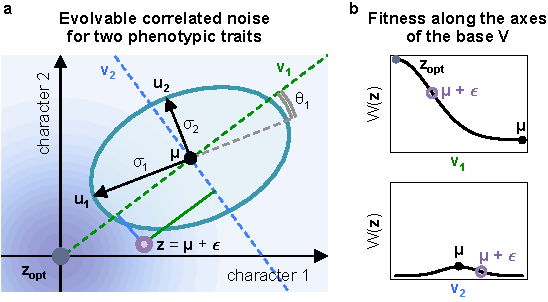
\includegraphics[scale=1.5]{part1_appendixS3_fig4.pdf}
\end{adjustwidth}
\caption[Anisotropic and correlated phenotypic noise for two traits.]{\textbf{Anisotropic and correlated phenotypic noise for two traits.}
\textbf{a,} The phenotypic distribution of an organism $(\boldsymbol{\mu}, \boldsymbol{\sigma}, \boldsymbol{\theta})$ is defined by a multivariate normal distribution with mean $\boldsymbol{\mu}$ (black dot), noise amplitudes $\sigma_1$ and $\sigma_2$ (black arrows) along axes $\boldsymbol{u_1}$ and $\boldsymbol{u_2}$, and a parameter of correlation $\theta_1$ (grey angle), defining a rotation of the basis $\boldsymbol{U} = (\boldsymbol{u_1}, \boldsymbol{u_2})$. A phenotype $\boldsymbol{z}$ (purple dot) is generated from the multivariate normal distribution by drawing a random vector $\boldsymbol{\epsilon} \sim \mathcal{N}_n(\boldsymbol{0},\boldsymbol{\Sigma})$ (with $\boldsymbol{\Sigma}$ the covariance matrix built from $\boldsymbol{\sigma}$ and $\boldsymbol{\theta}$), such that $\boldsymbol{z} = \boldsymbol{\mu} + \boldsymbol{\epsilon}$. The contribution of $\boldsymbol{\epsilon}$ on each axis $\boldsymbol{v_1}$ (in green) and $\boldsymbol{v_2}$ (in blue) of the basis $\boldsymbol{V}$, where $\boldsymbol{v_1}$ is aligned with the fitness optimum $\boldsymbol{z_{opt}}$, is represented by the vector $\boldsymbol{s} = (s_1, s_2)^T$. The fitness landscape is represented by a gradient of blue centered on the fitness optimum $\boldsymbol{z_{opt}}$ (blue dot).
\textbf{b,} Fitness along axes of the basis $\boldsymbol{V} = (\boldsymbol{v_1}, \boldsymbol{v_2})$. Along axis $\boldsymbol{v_1}$, aligned with the fitness optimum $\boldsymbol{z_{opt}}$, the organism experiences a convex fitness (if $\lVert \boldsymbol{\mu} \rVert > 1$). Along axis $\boldsymbol{v_2}$, orthogonal to $\boldsymbol{v_1}$, the organism a concave fitness, sitting on a local fitness optimum.
}
\label{part1:appendixS3:fig4}
\end{figure}

%%%%%%%%%%%%%%%%%
%%%%%%%%%%%%%%%%%

\section*{Concluding remarks}

Our demonstrations mainly rely on the study of the local convexity of the fitness function. As such, any function admitting the same properties as $W(\boldsymbol{z})=\exp\left[-\boldsymbol{z}^2/2\right]$ (\textit{i.e.}, a positive function being concave at the optimum and admitting one convex inflection point) will give the same general results. Moreover, in our study, phenotypic noise and mutation distributions are Gaussian-shaped. As demonstrated above, this choice allowed us to obtain precise analytical results.



\newpage

%%%%%%%%%%%%%%%%%%%%%%%%%%%

\subsection{Data S1. Phenotypic noise correlations matrices of each replicate of the 37 strains of yeast in Fisher's space.}
\label{part1:DataS1}

\href{https://github.com/charlesrocabert/SigmaFGM/tree/master/phenomics\_analysis/DataS1.zip}{https://github.com/charlesrocabert/SigmaFGM/tree/master/phenomics\_analysis/DataS1.zip}

\newpage

%%%%%%%%%%%%%%%%%%%%%%%%%%%

\subsection{Data S2. Phenotypic noise correlations matrices of each of the 37 strains of yeast in Fisher's space, with Pearson correlation tests.}
\label{part1:DataS2}

\href{https://github.com/charlesrocabert/SigmaFGM/tree/master/phenomics\_analysis/DataS1.zip}{https://github.com/charlesrocabert/SigmaFGM/tree/master/phenomics\_analysis/DataS2.zip}

\newpage

%%%%%%%%%%%%%%%%%%%%%%%%%%%

\subsection{Script S1. A numerical solver for {\sigmaFGM}.}
\label{part1:ScriptS1}

\href{https://github.com/charlesrocabert/SigmaFGM}{https://github.com/charlesrocabert/SigmaFGM}

\newpage

%%%%%%%%%%%%%%%%%%%%%%%%%%%

\subsection{Script S2. Phenomics analysis of 37 strains of yeast.}
\label{part1:ScriptS2}

\href{https://github.com/charlesrocabert/SigmaFGM/tree/master/phenomics\_analysis}{https://github.com/charlesrocabert/SigmaFGM/tree/master/phenomics\_analysis}

\newpage

%%%%%%%%%%%%%%%%%%%%%%%%%%%







